% GENERATED by scripts/make_supplementary_tables.py from git 7c55fbc (verbatim text; references resolved, floats in the v5 supplementary material left out: tab:c2_classify, tab:c2_custody, tab:c2_partitions, tab:c2_targets, tab:main)
\section*{From the Supplementary Material of Version 7c55fbc}

This document collects results that support statements of the paper but are
not needed to follow its argument. Section~\ref{app:heldout} reports additional
analyses of the held-out period of the earlier evaluation, performed after its
main results were known; Section~\ref{supp:reanalysis} reanalyses that period in
the format of the confirmation experiment; and Section~\ref{supp:confirm2diag}
gives per-block curves, diagnostics, and the tuning history and trial run of the
confirmation experiment.
% v4 S11: the earlier sentence "All results are additional analyses, performed
% after the main results on the held-out period were known" no longer held once
% the confirmation diagnostics and the pre-lock tuning history were added.
Fig.~\ref{fig:group_recall_A} and Table~\ref{tab:worst_groups} complement the
main results on the held-out period. Tables~\ref{tab:outage_expl1}
and~\ref{tab:outage_expl2} give the full outage results on the exploratory
periods, Table~\ref{tab:outage_early} covers the first 48~h after the outage start
on the held-out period, Table~\ref{tab:lost_hops} decomposes the hops affected by
the outage, Table~\ref{tab:ceiling} reports the share of hops below the most
permissive threshold of \texttt{mvp\_log}, and Tables~\ref{tab:oracle_groups}
and~\ref{tab:extra_cost} compare \texttt{mvp\_log} with the hindsight oracle of
the same outage scenario, by group and by hop type.

\begin{figure*}[!htb]
\centering
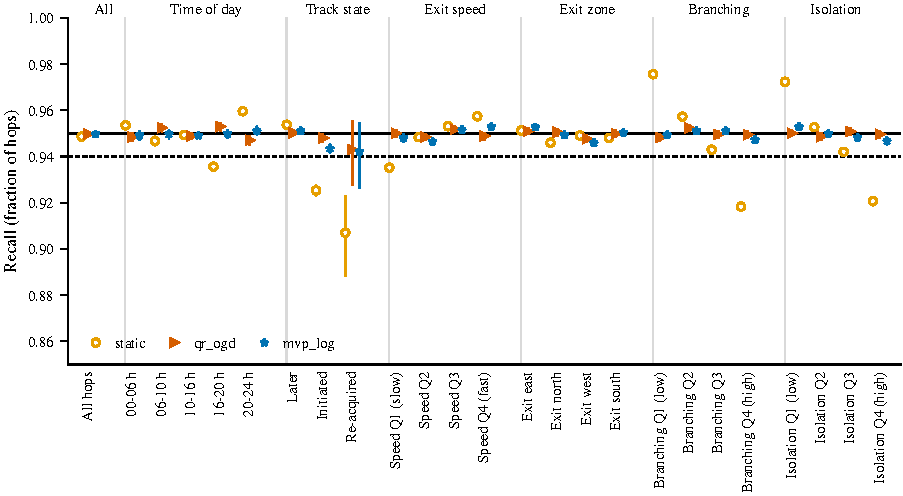
\includegraphics[width=\textwidth]{generated/figures/fig_group_recall_A.pdf}
\caption{Recall per group on held-out segment~A, in the format of
Fig.~\ref{fig:group_recall}.}
\label{fig:group_recall_A}
\end{figure*}

\begin{figure*}[!t]
\centering
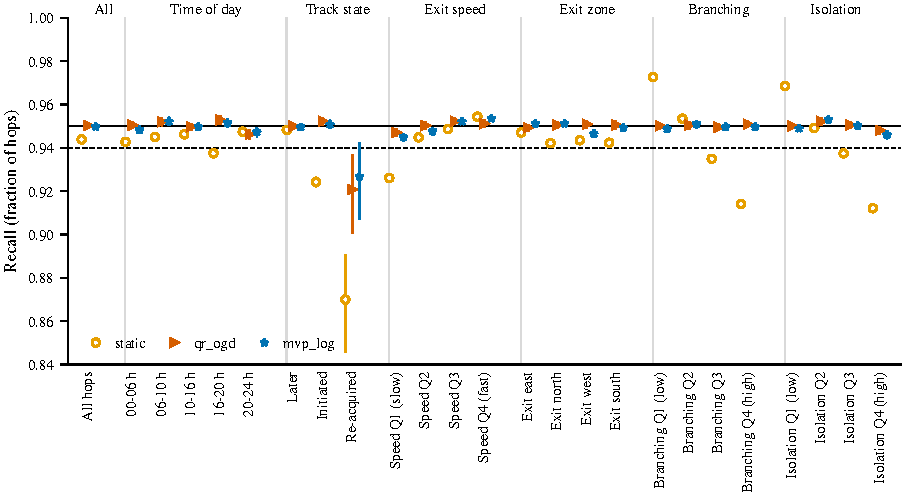
\includegraphics[width=\textwidth]{generated/figures/fig_group_recall_B.pdf}
\caption{Recall per group on held-out segment~B for split conformal calibration
(\texttt{static}), \texttt{qr\_ogd}, and \texttt{mvp\_log}, with 95\% Wilson
intervals. Groups are
ordered by attribute; isolation is the distance from the source site to the
nearest other site. Solid line: target \targetRecall; dashed line: bar
\groupBar. Segment~A is shown in Fig.~\ref{fig:group_recall_A}.}
\label{fig:group_recall}
\end{figure*}

\begin{table*}[t]
\centering
\caption{Worst group of each method on the held-out period (evaluation seed~0):
group, recall, number of hops $n$, and 95\% Wilson interval.
$^\dagger$Added after the main results were known.}
\label{tab:worst_groups}
\footnotesize
% AUTO-GENERATED by scripts/make_tables.py -- DO NOT EDIT. Data: generated/data/tab_worst_groups.csv
\begin{tabular}{l lrrc lrrc}
\toprule
& \multicolumn{4}{c}{Segment A} & \multicolumn{4}{c}{Segment B} \\
\cmidrule(lr){2-5}\cmidrule(lr){6-9}
Method & Group & Recall & $n$ & 95\% CI & Group & Recall & $n$ & 95\% CI \\
\midrule
static & Re-acquired & 0.907 & 1{,}054 & [0.888, 0.923] & Re-acquired & 0.870 & 846 & [0.846, 0.891] \\
ACI & Re-acquired & 0.904 & 1{,}054 & [0.885, 0.921] & Re-acquired & 0.881 & 846 & [0.857, 0.901] \\
Mondrian & Branching Q4 (high) & 0.919 & 66{,}829 & [0.917, 0.921] & Re-acquired & 0.885 & 846 & [0.862, 0.905] \\
Spatula-style & Re-acquired & 0.825 & 1{,}054 & [0.801, 0.847] & Re-acquired & 0.824 & 846 & [0.797, 0.848] \\
CityTrac-style (0.95)$^\dagger$ & Speed Q1 (slow) & 0.945 & 63{,}228 & [0.943, 0.947] & Re-acquired & 0.933 & 846 & [0.914, 0.948] \\
CityTrac-style (0.99)$^\dagger$ & Speed Q1 (slow) & 0.963 & 63{,}228 & [0.961, 0.964] & Re-acquired & 0.956 & 846 & [0.940, 0.968] \\
qr\_groups & Re-acquired & 0.942 & 1{,}054 & [0.926, 0.955] & Re-acquired & 0.915 & 846 & [0.894, 0.932] \\
mvp\_groups & Re-acquired & 0.942 & 1{,}054 & [0.926, 0.955] & Re-acquired & 0.931 & 846 & [0.912, 0.947] \\
mvp\_global & Re-acquired & 0.906 & 1{,}054 & [0.887, 0.922] & Re-acquired & 0.877 & 846 & [0.853, 0.898] \\
qr\_ogd & Re-acquired & 0.943 & 1{,}054 & [0.927, 0.956] & Re-acquired & 0.921 & 846 & [0.901, 0.937] \\
mvp\_log & Re-acquired & 0.942 & 1{,}054 & [0.926, 0.955] & Re-acquired & 0.927 & 846 & [0.907, 0.942] \\
hindsight oracle & Re-acquired & 0.909 & 1{,}054 & [0.890, 0.925] & Re-acquired & 0.876 & 846 & [0.852, 0.896] \\
\bottomrule
\end{tabular}

\end{table*}

\begin{table*}[t]
\centering
\caption{Camera outages on exploratory period~1, in the format of
Table~\ref{tab:outage}, from 48~h after the outage start, which is the start of
the period's second evaluation segment, to the end of its last evaluation
segment. In this period, the second segment is the Christmas and New Year holiday
period, so the outage starts together with the holidays.}
\label{tab:outage_expl1}
\footnotesize
% AUTO-GENERATED by scripts/make_tables.py -- DO NOT EDIT. Data: generated/data/tab_outage_expl1.csv
\begin{tabular}{@{}ll rrr rrr rrr rrr@{}}
\toprule
& & \multicolumn{3}{c}{static} & \multicolumn{3}{c}{ACI} & \multicolumn{3}{c}{qr\_ogd} & \multicolumn{3}{c}{mvp\_log} \\
\cmidrule(lr){3-5}\cmidrule(lr){6-8}\cmidrule(lr){9-11}\cmidrule(lr){12-14}
Outage & Pred. & Recall & $<$0.94 & Cost & Recall & $<$0.94 & Cost & Recall & $<$0.94 & Cost & Recall & $<$0.94 & Cost \\
\midrule
Random 10\% & base & 0.871 & 24.8 & 0.89 & 0.950 & 5.0 & 28.13 & 0.938 & 11.4 & 10.88 & 0.936 & 12.8 & 16.27 \\
 & aware & 0.928 & 19.4 & 1.01 & 0.950 & 4.8 & 1.71 & 0.950 & 1.2 & 1.87 & 0.951 & 0.6 & 2.07 \\
Random 20\% & base & 0.823 & 25.0 & 0.81 & 0.950 & 4.0 & 52.08 & 0.924 & 20.4 & 21.70 & 0.926 & 18.0 & 24.44 \\
 & aware & 0.904 & 24.0 & 0.99 & 0.950 & 5.0 & 2.92 & 0.950 & 1.6 & 3.17 & 0.948 & 1.4 & 3.52 \\
Random 30\% & base & 0.763 & 25.0 & 0.75 & 0.950 & 5.2 & 65.48 & 0.912 & 23.4 & 32.94 & 0.902 & 20.4 & 29.35 \\
 & aware & 0.880 & 24.8 & 1.00 & 0.950 & 3.6 & 4.09 & 0.950 & 2.2 & 4.10 & 0.948 & 0.8 & 4.54 \\
Region (20 sites) & base & 0.937 & 11 & 0.95 & 0.950 & 6 & 1.49 & 0.949 & 3 & 1.57 & 0.947 & 4 & 3.52 \\
 & aware & 0.938 & 10 & 0.96 & 0.950 & 6 & 1.46 & 0.950 & 3 & 1.60 & 0.951 & 1 & 2.11 \\
\bottomrule
\end{tabular}

\end{table*}

\begin{table*}[t]
\centering
\caption{Camera outages on exploratory period~2, in the format of
Table~\ref{tab:outage}, from 48~h after the outage start to the end of the
period's last evaluation segment.}
\label{tab:outage_expl2}
\footnotesize
% AUTO-GENERATED by scripts/make_tables.py -- DO NOT EDIT. Data: generated/data/tab_outage_expl2.csv
\begin{tabular}{@{}ll rrr rrr rrr rrr@{}}
\toprule
& & \multicolumn{3}{c}{static} & \multicolumn{3}{c}{ACI} & \multicolumn{3}{c}{qr\_ogd} & \multicolumn{3}{c}{mvp\_log} \\
\cmidrule(lr){3-5}\cmidrule(lr){6-8}\cmidrule(lr){9-11}\cmidrule(lr){12-14}
Outage & Pred. & Recall & $<$0.94 & Cost & Recall & $<$0.94 & Cost & Recall & $<$0.94 & Cost & Recall & $<$0.94 & Cost \\
\midrule
Random 10\% & base & 0.868 & 25.0 & 0.86 & 0.950 & 5.2 & 33.84 & 0.941 & 8.6 & 16.40 & 0.933 & 14.8 & 15.44 \\
 & aware & 0.923 & 22.2 & 0.98 & 0.950 & 5.2 & 1.92 & 0.950 & 0.6 & 2.44 & 0.950 & 0.2 & 2.48 \\
Random 20\% & base & 0.821 & 25.0 & 0.79 & 0.950 & 5.4 & 54.59 & 0.931 & 15.0 & 30.35 & 0.921 & 20.4 & 22.04 \\
 & aware & 0.903 & 24.6 & 0.96 & 0.950 & 4.2 & 2.92 & 0.950 & 0.8 & 3.68 & 0.949 & 0.2 & 3.81 \\
Random 30\% & base & 0.759 & 25.0 & 0.72 & 0.950 & 5.2 & 72.29 & 0.920 & 18.0 & 44.23 & 0.890 & 22.8 & 25.11 \\
 & aware & 0.876 & 25.0 & 0.96 & 0.950 & 4.0 & 4.82 & 0.949 & 0.4 & 5.07 & 0.949 & 0.0 & 5.26 \\
Region (20 sites) & base & 0.933 & 17 & 0.92 & 0.950 & 6 & 1.61 & 0.949 & 3 & 1.97 & 0.944 & 5 & 3.04 \\
 & aware & 0.934 & 17 & 0.93 & 0.950 & 6 & 1.56 & 0.949 & 2 & 2.03 & 0.949 & 0 & 2.82 \\
\bottomrule
\end{tabular}

\end{table*}

\begin{table*}[t]
\centering
\caption{Camera outages on the held-out period during the first 48~h after the
outage start, in the format of Table~\ref{tab:outage}.}
\label{tab:outage_early}
\footnotesize
% AUTO-GENERATED by scripts/make_tables.py -- DO NOT EDIT. Data: generated/data/tab_outage_early.csv
\begin{tabular}{@{}ll rrr rrr rrr rrr@{}}
\toprule
& & \multicolumn{3}{c}{static} & \multicolumn{3}{c}{ACI} & \multicolumn{3}{c}{qr\_ogd} & \multicolumn{3}{c}{mvp\_log} \\
\cmidrule(lr){3-5}\cmidrule(lr){6-8}\cmidrule(lr){9-11}\cmidrule(lr){12-14}
Outage & Pred. & Recall & $<$0.94 & Cost & Recall & $<$0.94 & Cost & Recall & $<$0.94 & Cost & Recall & $<$0.94 & Cost \\
\midrule
Random 10\% & base & 0.869 & 23.8 & 0.94 & 0.950 & 4.2 & 42.89 & 0.912 & 20.4 & 3.65 & 0.896 & 23.4 & 5.63 \\
 & aware & 0.928 & 17.8 & 1.07 & 0.949 & 3.0 & 1.83 & 0.944 & 3.6 & 1.77 & 0.929 & 16.0 & 1.48 \\
Random 20\% & base & 0.828 & 24.0 & 0.85 & 0.951 & 3.8 & 55.89 & 0.887 & 23.8 & 5.15 & 0.874 & 24.0 & 8.99 \\
 & aware & 0.909 & 22.0 & 1.04 & 0.951 & 1.4 & 2.81 & 0.940 & 5.2 & 2.34 & 0.913 & 21.2 & 1.63 \\
Random 30\% & base & 0.767 & 24.0 & 0.79 & 0.950 & 3.8 & 84.06 & 0.845 & 24.0 & 6.43 & 0.835 & 24.0 & 12.37 \\
 & aware & 0.884 & 23.6 & 1.05 & 0.950 & 2.8 & 4.75 & 0.933 & 12.0 & 2.87 & 0.897 & 23.4 & 1.92 \\
Region (20 sites) & base & 0.938 & 8 & 1.01 & 0.948 & 5 & 1.44 & 0.944 & 4 & 1.38 & 0.937 & 8 & 1.23 \\
 & aware & 0.939 & 8 & 1.02 & 0.947 & 5 & 1.40 & 0.944 & 4 & 1.42 & 0.938 & 5 & 1.26 \\
\bottomrule
\end{tabular}

\end{table*}

\begin{table*}[t]
\centering
\caption{Hops affected by camera outages on held-out segment~B (original
predictor's hop set without outage as reference). Removed: hops whose source site
failed, and hops that became exits. Rerouted: hops whose object re-appears at a
later site after skipping one or more failed sites. Recall of rerouted hops for
\texttt{mvp\_log} with the original and the outage-aware predictor. Random
outages: one of the five draws of failed sites, the one used in the first outage
experiments; Region: an earlier local outage of six sites.}
\label{tab:lost_hops}
\footnotesize
% AUTO-GENERATED by scripts/make_tables.py -- DO NOT EDIT. Data: generated/data/tab_lost_hops.csv
\begin{tabular}{l r rr rr rr}
\toprule
& & \multicolumn{2}{c}{Removed (\%)} & \multicolumn{2}{c}{Rerouted (\%)} & \multicolumn{2}{c}{Recall, rerouted} \\
\cmidrule(lr){3-4}\cmidrule(lr){5-6}\cmidrule(lr){7-8}
Outage & Sites off & Source off & To exit & Skip 1 & Skip $\geq$2 & Base & Outage-aware \\
\midrule
Random 10\% & 18 & 11.7 & 1.5 & 6.3 & 1.8 & 0.275 & 0.793 \\
Random 20\% & 35 & 20.3 & 4.1 & 10.6 & 1.4 & 0.580 & 0.811 \\
Random 30\% & 53 & 26.4 & 5.0 & 7.2 & 3.5 & 0.485 & 0.738 \\
Region (6 sites) & 6 & 4.6 & 0.4 & 0.6 & 0.7 & 0.086 & 0.506 \\
\bottomrule
\end{tabular}

\end{table*}

\begin{table*}[t]
\centering
\caption{Share of hops whose score lies below the most permissive threshold
$\tau_{\min}$ of \texttt{mvp\_log}, by group, from 48~h after the outage start
(held-out period, mean over five draws of failed sites). $^\dagger$Above
$\alpha=0.05$, i.e., the target is infeasible for this group
(Section~\ref{M-sec:method:mvp}).}
\label{tab:ceiling}
\footnotesize
% AUTO-GENERATED by scripts/make_tables.py -- DO NOT EDIT. Data: generated/data/tab_ceiling.csv
\begin{tabular}{l rr rr}
\toprule
& \multicolumn{2}{c}{Random 10\%} & \multicolumn{2}{c}{Random 30\%} \\
\cmidrule(lr){2-3}\cmidrule(lr){4-5}
Group & Base & Outage-aware & Base & Outage-aware \\
\midrule
All hops & 0.050 & 0.001 & 0.109$^\dagger$ & 0.001 \\
\addlinespace[2pt]
00-06 h & 0.056$^\dagger$ & 0.001 & 0.119$^\dagger$ & 0.001 \\
06-10 h & 0.052$^\dagger$ & 0.001 & 0.112$^\dagger$ & 0.001 \\
10-16 h & 0.050 & 0.001 & 0.111$^\dagger$ & 0.001 \\
16-20 h & 0.047 & 0.001 & 0.102$^\dagger$ & 0.001 \\
20-24 h & 0.043 & 0.001 & 0.099$^\dagger$ & 0.001 \\
\addlinespace[2pt]
Later & 0.051$^\dagger$ & 0.001 & 0.105$^\dagger$ & 0.001 \\
Initiated & 0.046 & 0.001 & 0.123$^\dagger$ & 0.002 \\
Re-acquired & 0.062$^\dagger$ & 0.001 & 0.123$^\dagger$ & 0.004 \\
\addlinespace[2pt]
Speed Q1 (slow) & 0.033 & 0.001 & 0.096$^\dagger$ & 0.001 \\
Speed Q2 & 0.038 & 0.001 & 0.098$^\dagger$ & 0.001 \\
Speed Q3 & 0.049 & 0.001 & 0.115$^\dagger$ & 0.001 \\
Speed Q4 (fast) & 0.084$^\dagger$ & 0.001 & 0.131$^\dagger$ & 0.001 \\
\addlinespace[2pt]
Exit east & 0.037 & 0.001 & 0.098$^\dagger$ & 0.001 \\
Exit north & 0.059$^\dagger$ & 0.001 & 0.108$^\dagger$ & 0.001 \\
Exit west & 0.064$^\dagger$ & 0.001 & 0.136$^\dagger$ & 0.002 \\
Exit south & 0.040 & 0.001 & 0.098$^\dagger$ & 0.001 \\
\addlinespace[2pt]
Branching Q1 (low) & 0.054$^\dagger$ & 0.001 & 0.116$^\dagger$ & 0.001 \\
Branching Q2 & 0.040 & 0.001 & 0.101$^\dagger$ & 0.001 \\
Branching Q3 & 0.052$^\dagger$ & 0.001 & 0.112$^\dagger$ & 0.003 \\
Branching Q4 (high) & 0.052$^\dagger$ & 0.002 & 0.106$^\dagger$ & 0.001 \\
\addlinespace[2pt]
Isolation Q1 (low) & 0.050$^\dagger$ & 0.001 & 0.091$^\dagger$ & 0.001 \\
Isolation Q2 & 0.032 & 0.001 & 0.088$^\dagger$ & 0.001 \\
Isolation Q3 & 0.062$^\dagger$ & 0.002 & 0.153$^\dagger$ & 0.001 \\
Isolation Q4 (high) & 0.061$^\dagger$ & 0.002 & 0.123$^\dagger$ & 0.002 \\
\bottomrule
\end{tabular}

\end{table*}

\begin{table}[t]
\centering
\caption{Recall per group of \texttt{mvp\_log} and of the hindsight oracle of the
same scenario, and the cost of \texttt{mvp\_log} relative to that oracle, under a
random outage of 10\% of the sites with the outage-aware predictor (held-out
period, from 48~h after the outage start; one of the five draws of failed sites,
the one used in the first outage experiments).}
\label{tab:oracle_groups}
\footnotesize
% AUTO-GENERATED by scripts/make_tables.py -- DO NOT EDIT. Data: generated/data/tab_oracle_groups.csv
\begin{tabular}{l r rr r}
\toprule
& & \multicolumn{2}{c}{Recall} & \\
\cmidrule(lr){3-4}
Group & $n$ & mvp\_log & Oracle & Cost ratio \\
\midrule
All hops & 167{,}979 & 0.947 & 0.950 & 1.54 \\
\addlinespace[2pt]
00-06 h & 37{,}293 & 0.943 & 0.949 & 1.82 \\
06-10 h & 26{,}930 & 0.948 & 0.945 & 1.79 \\
10-16 h & 48{,}306 & 0.950 & 0.951 & 1.48 \\
16-20 h & 30{,}140 & 0.949 & 0.949 & 1.30 \\
20-24 h & 25{,}310 & 0.944 & 0.956 & 1.41 \\
\addlinespace[2pt]
Later & 134{,}749 & 0.947 & 0.952 & 1.42 \\
Initiated & 32{,}517 & 0.951 & 0.945 & 1.89 \\
Re-acquired & 713 & 0.913 & 0.853 & 5.50 \\
\addlinespace[2pt]
Speed Q1 (slow) & 41{,}581 & 0.948 & 0.955 & 1.08 \\
Speed Q2 & 45{,}841 & 0.951 & 0.966 & 0.92 \\
Speed Q3 & 43{,}534 & 0.945 & 0.962 & 1.13 \\
Speed Q4 (fast) & 37{,}023 & 0.945 & 0.910 & 3.99 \\
\addlinespace[2pt]
Exit east & 46{,}714 & 0.952 & 0.965 & 0.98 \\
Exit north & 44{,}111 & 0.941 & 0.942 & 1.60 \\
Exit west & 39{,}162 & 0.948 & 0.925 & 2.83 \\
Exit south & 37{,}992 & 0.948 & 0.967 & 0.82 \\
\addlinespace[2pt]
Branching Q1 (low) & 43{,}353 & 0.940 & 0.983 & 0.28 \\
Branching Q2 & 40{,}090 & 0.949 & 0.934 & 2.19 \\
Branching Q3 & 44{,}233 & 0.950 & 0.937 & 2.16 \\
Branching Q4 (high) & 40{,}303 & 0.950 & 0.945 & 1.44 \\
\addlinespace[2pt]
Isolation Q1 (low) & 49{,}550 & 0.942 & 0.982 & 0.34 \\
Isolation Q2 & 46{,}136 & 0.955 & 0.973 & 0.58 \\
Isolation Q3 & 38{,}376 & 0.946 & 0.944 & 1.58 \\
Isolation Q4 (high) & 33{,}917 & 0.945 & 0.879 & 4.23 \\
\bottomrule
\end{tabular}

\end{table}

\begin{table}[t]
\centering
\caption{Extra cost of \texttt{mvp\_log} relative to the hindsight oracle of the
same scenario, by hop type, under a random outage of 10\% of the sites with the
outage-aware predictor (held-out period, from 48~h after the outage start; one of
the five draws of failed sites, the one used in the first outage experiments).
Share of hops, recall of both rules, and share of the extra cost.}
\label{tab:extra_cost}
\footnotesize
% AUTO-GENERATED by scripts/make_tables.py -- DO NOT EDIT. Data: generated/data/tab_extra_cost.csv
\begin{tabular}{@{}p{2.9cm} rrrr@{}}
\toprule
Hop type & Hops & \multicolumn{2}{c}{Recall} & Extra \\
\cmidrule(lr){3-4}
 & (\%) & mvp\_log & Oracle & cost (\%) \\
\midrule
Not rerouted & 90.5 & 0.962 & 0.972 & 15.1 \\
Rerouted, 1 failed site skipped & 7.2 & 0.882 & 0.927 & 16.5 \\
Rerouted, $\ge$2 failed sites skipped & 2.1 & 0.574 & 0.083 & 68.2 \\
New (source episode changed) & 0.1 & 0.293 & 0.992 & -0.5 \\
Re-acquisition caused by the outage & 0.1 & 0.919 & 0.892 & 0.7 \\
\midrule
All & 100.0 & 0.947 & 0.950 & 100.0 \\
\bottomrule
\end{tabular}

\end{table}

% ---------------------------------------------------------------------
% Moved from the main appendix (JD approval 2026-10-18; David v3 instruction section 6): former Appendix B.
% Labels unchanged; references to the main text use the prefix M-.
\section{Additional Analyses on the Held-Out Period}
\label{app:heldout}

All analyses in this section were performed on the held-out period of
Appendix~\ref{app:earlier} after its results were known. None of them includes the
refitted comparators of the confirmation experiment; in particular, the outage
analyses do not compare online updating with refitting, and we do not use them
as evidence for online updating.

\subsection{Robustness}
\label{app:earlier:robust}
\label{app:earlier:seeds}
\label{app:earlier:custody}
\label{app:earlier:ablation}
\label{app:earlier:sensitivity}

\paragraph*{Evaluation seeds}
Over \seedCount{} evaluation seeds, including that of the main results, the group
criterion holds for \texttt{mvp\_log} in \seedCOnePassMvpLog{} and for
\texttt{qr\_ogd} in \seedCOnePassQrOgd{}, and the cost criterion in all
(Table~\ref{tab:seeds}). Every failure is a single group, the re-acquisition hops
in segment~B (recall \seedReacqMvpLogMin{} to \seedReacqMvpLogMax{} for
\texttt{mvp\_log}). This group contains about \reacqSharePct\% of the hops, so few
feedback hops fall into it; it is the persistent weak point of both methods.

\paragraph*{Observation radius and horizon}
Repeating the evaluation with observation radii of \geomRadiusSmall{} and
\geomRadiusLarge~m and horizons of \geomTmaxShort{} and \geomTmaxLong~s, with
hops, groups, and models rebuilt (Table~\ref{tab:geometry}), marginal calibration
fails in every setting (\geomMarginalBelowMin{} to \geomMarginalBelowMax{} groups
below the bar). The multigroup methods meet the group criterion in most seeds of
most settings, at mean costs of \geomMultiCostSeedMeanMin{} to
\geomMultiCostSeedMeanMax{} times the oracle, but not uniformly: with the
\geomTmaxLong-s horizon, \texttt{mvp\_log} fails in all \geomSeedCountWord{} seeds,
on the re-acquisition group, whereas \texttt{qr\_ogd} meets the group criterion in
\geomTmaxLongQrOgdPassWord{} at a cost of \geomTmaxLongQrOgdCostMin{} to
\geomTmaxLongQrOgdCostMax{} times the oracle, and both criteria in only one. We did
not investigate why. Neither instance dominates the other across settings.

\paragraph*{Threshold scale}
On the exploratory periods (Table~\ref{tab:ablation}), the logarithmic scale
reduces the cost from \ablUnifNoCapRatioMean{} to \ablLogCapRatioMean{} times the
oracle; the finer grid accounts for \ablResolutionSharePctFirst\% and
\ablResolutionSharePctSecond\% of the reduction in the two periods and the bound
$a_{\min}$ for the rest. With the logarithmic grid, removing the bound changes the
cost only to \ablLogNoCapMatchedRatioMean{} but, like $a_{\min}=\aMinHigh$, leads to
one exploratory segment with a group below the bar.

% verbatim from 7c55fbc sections/sec4_method.tex (observed target under imperfect detection)
\paragraph*{Detection target (Section IV of version 7c55fbc)}
To target a true recall of $1-\alpha$, the observed
target is set to
\begin{equation}
  1-\alpha_{\mathrm{obs}} = (1-\alpha)\,p_{\mathrm{det}},
  \label{eq:det-target}
\end{equation}
which requires an estimate of $p_{\mathrm{det}}$ for the deployed detector.

\paragraph*{Feedback and detection}
The results hardly depend on the feedback model
(Table~\ref{tab:sensitivity}): with \sensFeedbackMinPct\% to
\sensFeedbackMaxPct\% delayed feedback, at most one group (re-acquisition) falls
below the bar, at \sensFbCostRatioMin{} to \sensFbCostRatioMax{} times the oracle
cost. Imperfect detection matters: with detection probabilities of \sensDetHigh{}
and \sensDetLow{} and the target unchanged, the cost of \texttt{mvp\_log} rises to
\sensDetNinetyFiveUnadjCostRatio{} and \sensDetNinetyUnadjCostRatio{} times the
error-free oracle, whereas the adjusted target \eqref{eq:det-target} restores a
true recall of about \sensDetNinetyFiveAdjRecallA{} at
\sensDetNinetyFiveAdjCostRatio{} times for $p_{\mathrm{det}}=\sensDetHigh$, and of
\sensDetNinetyAdjRecallA{} for $p_{\mathrm{det}}=\sensDetLow$, with \sensDetNinetyAdjBelowBarMaxWord{} groups
below the bar in \sensDetNinetyAdjSegmentsBelowWord{} segment. Detection failures are assumed
independent.

\paragraph*{Track custody}
A track survives only if consecutive hops are all hit (Table~\ref{tab:custody}).
After five hops, \custFiveMinPct{} to \custFiveMaxPct\% of the chains survive under
every method, slightly more than independence would give, because consecutive hits
are positively correlated. Group-conditional calibration does not raise custody in
general: over all chains, the multigroup methods keep slightly fewer chains than
the oracle and ACI, because on later hops, which make up most of a chain, their
recall is \custLaterRecallGapMin{} to \custLaterRecallGapMax{} points lower
(Table~\ref{tab:group_oracle}, lower part). For chains that start with a
re-acquisition,
\texttt{mvp\_log} raises the first-hop recall (\custReacqMvpLogBKOne{} against
\custReacqOracleBKOne{} in segment~B), but over five hops the effect is mixed. A
custody target thus requires a higher per-hop target, which we did not evaluate.

\begin{figure*}[!t]
\centering
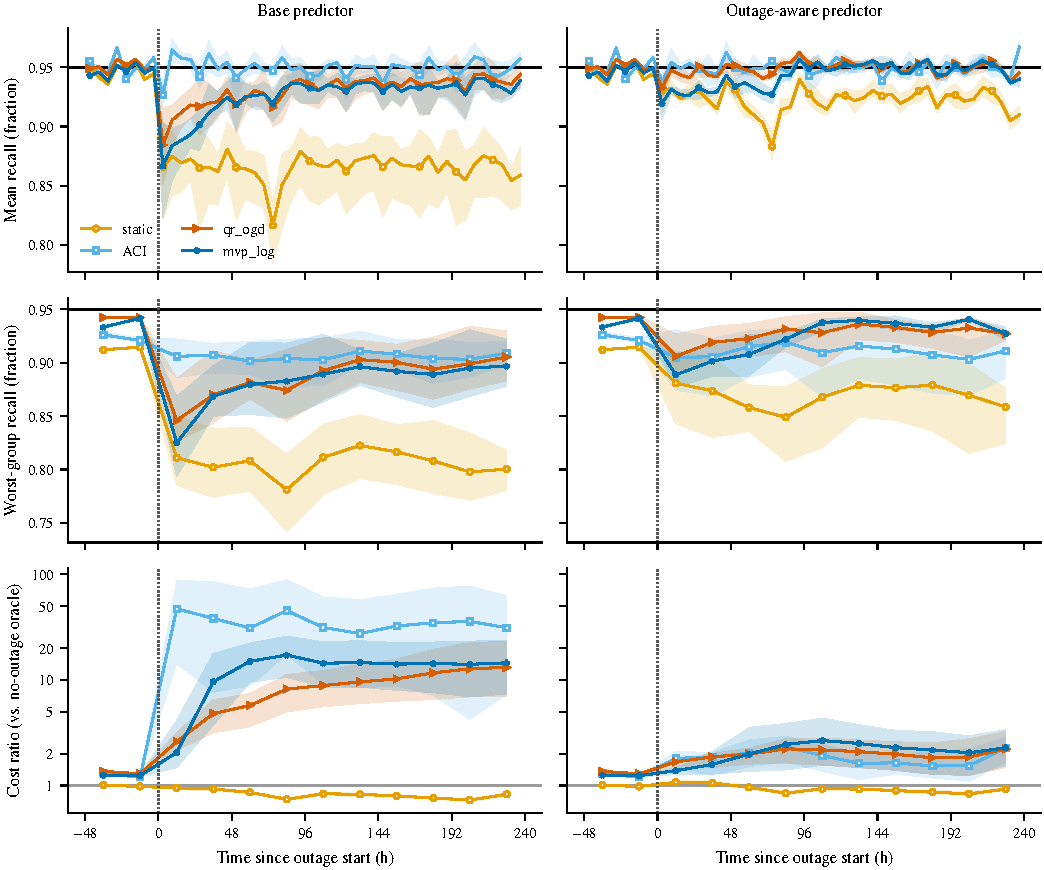
\includegraphics[width=\textwidth]{generated/figures/fig_outage_timeseries.pdf}
\caption{Recall and cost over time under a random outage of 10\% of the sites on
the held-out period (additional analysis). Lines: mean over five draws of failed
sites; bands: minimum to maximum. Top: mean recall (6-h bins). Middle: worst-group
recall (24-h bins, groups with at least \minGroupHops hops). Bottom: cost relative
to the mean cost of the hindsight oracle without outage in the same segment
(24-h bins, logarithmic axis). Left: original predictor; right: outage-aware
predictor.}
\label{fig:outage}
\end{figure*}

\subsection{Camera Outages}
\label{app:earlier:outage}

From the start of segment~B, a random 10\%, 20\%, or 30\% of the sites, or the
\regionSites{} sites around the busiest site, stop operating
(Fig.~\ref{fig:outage}, Table~\ref{tab:outage}; additional analysis).

\paragraph*{Original predictor}
No calibration rule maintains group recall at a reasonable cost. Under the 10\%
outage, \texttt{mvp\_log} reaches \outTenBaseMvpLogRecall{} with
\outTenBaseMvpLogBelowBar{} groups below the bar at \outTenBaseMvpLogCostRatio{}
times the cost of the oracle without outage; ACI keeps the mean at
\outTenBaseAciRecall{} only at \outTenBaseAciCostRatio{} times that cost; \texttt{static} falls to
\outTenBaseStaticRecall. The cause is the predictor: objects re-appear later and
farther away, at pairs never observed in training, and \texttt{mvp\_log} recalls
these rerouted hops at only \lostTenRelinkedRecallBase{}
(Table~\ref{tab:lost_hops}). The bound $a_{\min}$
turns this into a ceiling: the share of hops below $\tau_{\min}$ rises to
\ceilTenBaseAll{} and \ceilThirtyBaseAll{} under the 10\% and 30\% outages and
exceeds $\alpha$ in several groups, violating \eqref{eq:feasible}
(Table~\ref{tab:ceiling}); meanwhile, the share of hops assigned to the most
permissive threshold rises from zero to about one half. Lowering $a_{\min}$ helps only at
\outRandBaseMvpLogAMinLowCostMin{} to \outRandBaseMvpLogAMinLowCostMax{} times the
cost of the oracle without outage. In hindsight, the bound offers little in stationary conditions and
limits recovery under misspecification.

\paragraph*{Outage-aware predictor}
Replacing the predictor by one that composes transitions through failed sites,
developed after these results were known and replicated on the exploratory
periods (Table~\ref{tab:outage_expl}), restores most of the recall with every
calibration layer unchanged; the share of hops below $\tau_{\min}$ falls to
\ceilTenAwareAll{} under the 10\% outage. After the first 48~h, \texttt{mvp\_log} reaches
\outThirtyAwareMvpLogRecall{} to \outTenAwareMvpLogRecall{} with
\outTenAwareMvpLogBelowBar{} to \outThirtyAwareMvpLogBelowBar{} groups below the
bar, and \texttt{qr\_ogd} \outThirtyAwareQrOgdRecall{} to \outTenAwareQrOgdRecall{}
with \outThirtyAwareQrOgdBelowBar{} to \outTenAwareQrOgdBelowBar, at
\outTenAwareMvpLogCostRatio{} to \outThirtyAwareMvpLogCostRatio{} times the cost of
the oracle without outage; the extra cost of \texttt{mvp\_log} is concentrated on hops that skipped two
or more failed sites (Tables~\ref{tab:oracle_groups} and~\ref{tab:extra_cost}). The update does not settle
every case: when adjacent sites fail together, many rerouted hops skip several of
them, and \texttt{mvp\_log} still leaves \outRegionAwareMvpLogBelowBar{} groups
below the bar under the local outage. Once the predictor is updated, marginal ACI
leaves only \outThirtyAwareAciBelowBar{} to \outTenAwareAciBelowBar{} groups below
the bar, so the advantage of multigroup calibration is smaller than in stationary
conditions.

\paragraph*{The first 48 hours}
All methods fall short right after the outage. With the outage-aware predictor,
ACI and \texttt{qr\_ogd}, whose states move by constant steps, stay at or above a
mean recall of \groupBar{} for 24~h from \recovAwareFastHours~h after the start,
\texttt{mvp\_log} only from \recovAwareMvpLogHours~h (Table~\ref{tab:outage_early}).
Diagnostic runs support the mechanism of Section~\ref{M-sec:method:speed}: removing
the warm start shortened the recovery of MVP with a single group from
\warmMvpGlobalRecoverHours~h to \warmZeroMvpGlobalRecoverHours~h. The slow
transient is a limitation of \texttt{mvp\_log}. Under structural change, the
predictor must thus be updated; recalibration alone cannot compensate for a
predictor that does not know where objects re-appear.




All results in this section are additional analyses, performed after the main
results were known.

\paragraph*{List of additional analyses}
(i) \emph{CityTrac-style baseline}: added to the compared methods and evaluated on
the held-out period.
(ii) \emph{Evaluation seeds}: the held-out evaluation run with five seeds, including that of the main results, which change the feedback sample, the
randomization of MVP, and the calibration subsample of \texttt{qr\_groups}.
(iii) \emph{Cost-matched comparison} (Section~\ref{app:earlier:frontier}).
(iv) \emph{Sensitivity} to the feedback fraction (\sensFeedbackMinPct\% to \sensFeedbackMaxPct\%), to feedback delay,
and to imperfect detection, with detection probabilities between \sensDetLow and \sensDetHigh.
(v) \emph{Scale ablation} on the exploratory periods, separating the effect of the
logarithmic grid from that of the bound $a_{\min}$.
(vi) \emph{Camera outages}: from the start of the second evaluation segment, some
sites stop operating; sighting data of failed sites are removed and hops are
rebuilt, so that objects re-appear at the next operating site. We first ran
outages on the held-out period only (a random \initOutageRandLowPct\%, \initOutageRandMidPct\%, or \initOutageRandHighPct\% of the sites
drawn once, and a local outage of \initRegionSitesWord sites), followed by diagnostics of the
adaptation delay, including an ablation of the warm start, and a decomposition of
the hops lost or rerouted by the outage. We then ran random outages drawn with
\outageSiteSeedsWord seeds and a local outage of the \regionSites sites within a fixed radius of
the busiest site on all three periods. Rebuilding the hops changes the order in
which hops with the same exit time are processed, and hence the feedback sample,
slightly; before the outage, this changes the cost of \texttt{mvp\_log} by \outPreCostDiffMinPct\%
to \outPreCostDiffMaxPct\% across the outage runs.
(vii) \emph{Outage-aware predictor}: a variant of the predictor that composes
transitions through failed sites. We developed it after seeing the outage results
on the held-out period; it is therefore an extension informed by those results,
and we replicate its evaluation on the two exploratory periods.
(viii) \emph{Diagnostics of the bound $a_{\min}$}: the recall ceiling it imposes
under outages, the nature of the pairs below $\tau_{\min}$, and a per-group
comparison of cost with the hindsight oracle.
(ix) \emph{Group-conditional hindsight references}: two rules fitted in hindsight on
each held-out segment to meet the target in every group, used as cost references
(Section~\ref{app:earlier:main}).
(x) \emph{Track custody}: the share of chains whose first $k$ hops are all hit.
(xi) \emph{Geometry and horizon}: the held-out evaluation repeated, with five
evaluation seeds, for observation radii of \geomRadiusSmall and \geomRadiusLarge~m and horizons $T_{\max}$ of
\geomTmaxShort and \geomTmaxLong~s, with all hops, groups, and models rebuilt for each setting.

\paragraph*{Tables} Table~\ref{tab:seeds} lists the results of the two online
multigroup methods for each evaluation seed (Section~\ref{app:earlier:seeds}).
Table~\ref{tab:group_oracle} compares them with two references that meet the
target in every group in hindsight (Section~\ref{app:earlier:main}), and
Table~\ref{tab:custody} reports track custody over several hops
(Section~\ref{app:earlier:custody}). Table~\ref{tab:geometry} repeats the
held-out evaluation for other observation radii and horizons
(Section~\ref{app:earlier:sensitivity}). Table~\ref{tab:layout} compares the
attributes that matter on a synthetic and on the real camera layout
(Section~\ref{app:earlier:problem}), and Table~\ref{tab:outage_expl} replicates
the outage experiments with the outage-aware predictor on the exploratory periods
(Section~\ref{app:earlier:outage}).

\begin{table}[!htbp]
\centering
\caption{Spread of recall across the levels of each attribute under split
conformal calibration (maximum minus minimum over levels, percentage points), on
the two exploratory periods, for a synthetic layout of 130 sites placed by
traffic density and for the real CCTV layout (additional analysis). The two
layouts produce different hops.}
\label{tab:layout}
\footnotesize
% AUTO-GENERATED by scripts/make_tables.py -- DO NOT EDIT. Data: generated/data/tab_layout_factors.csv
\begin{tabular}{lrrrr}
\toprule
& \multicolumn{2}{c}{Synthetic layout} & \multicolumn{2}{c}{Real CCTV layout} \\
\cmidrule(lr){2-3}\cmidrule(lr){4-5}
Attribute & Period 1 & Period 2 & Period 1 & Period 2 \\
\midrule
Time of day & 1.1 & 1.7 & 1.4 & 1.6 \\
Track state & 6.1 & 6.5 & 6.5 & 5.5 \\
Exit speed & 8.2 & 8.0 & 3.2 & 2.6 \\
Exit zone & 2.4 & 2.2 & 0.5 & 1.0 \\
Branching & 6.4 & 7.1 & 5.2 & 5.3 \\
Isolation & 1.9 & 2.0 & 5.4 & 4.5 \\
\bottomrule
\end{tabular}

\end{table}

\begin{table*}[t]
\centering
\caption{Group-conditional references on the held-out period (evaluation
seed~0). (a) Group-minimum rule: each hop uses the lowest of the hindsight
thresholds of the groups that contain it. (b) Hindsight group QR: the quantile
regression of \texttt{qr\_groups} fitted on the evaluation segment itself. Cost in
camera-seconds per hop, and relative to the hindsight oracle and to rule~(a). The
lower part reports the later hops only, with costs relative to the hindsight
oracle on the same hops.}
\label{tab:group_oracle}
\footnotesize
% AUTO-GENERATED by scripts/make_tables.py -- DO NOT EDIT. Data: generated/data/tab_group_oracle.csv
\begin{tabular}{@{}ll rrlrr rrr@{}}
\toprule
Seg. & Reference / method & Recall & Worst & Worst group & $<$0.94 & $<$0.95 & Cost & $\times$oracle & $\times$(a) \\
\midrule
A & Hindsight oracle (global) & 0.950 & 0.909 & Re-acquired & 6 & 9 & 279 & 1.00 & 0.70 \\
 & Group-minimum rule (a) & 0.964 & 0.950 & Isolation Q4 (high) & 0 & 0 & 400 & 1.44 & 1.00 \\
 & Hindsight group QR (b) & 0.950 & 0.950 & Exit south & 0 & 0 & 330 & 1.18 & 0.82 \\
 & qr\_ogd & 0.950 & 0.943 & Re-acquired & 0 & 3 & 334 & 1.20 & 0.83 \\
 & mvp\_log & 0.950 & 0.942 & Re-acquired & 0 & 7 & 330 & 1.18 & 0.82 \\
\addlinespace[2pt]
B & Hindsight oracle (global) & 0.950 & 0.876 & Re-acquired & 5 & 8 & 301 & 1.00 & 0.69 \\
 & Group-minimum rule (a) & 0.964 & 0.950 & Re-acquired & 0 & 0 & 436 & 1.45 & 1.00 \\
 & Hindsight group QR (b) & 0.950 & 0.950 & 00-06 h & 0 & 0 & 357 & 1.18 & 0.82 \\
 & qr\_ogd & 0.950 & 0.921 & Re-acquired & 1 & 4 & 356 & 1.18 & 0.82 \\
 & mvp\_log & 0.950 & 0.927 & Re-acquired & 0 & 7 & 353 & 1.17 & 0.81 \\
\midrule
\multicolumn{10}{@{}l}{\emph{Later hops only}} \\
A & Hindsight oracle (global) & 0.955 & -- &  & -- & -- & 270 & 1.00 & -- \\
 & ACI & 0.955 & -- &  & -- & -- & 290 & 1.07 & -- \\
 & qr\_ogd & 0.950 & -- &  & -- & -- & 296 & 1.09 & -- \\
 & mvp\_log & 0.951 & -- &  & -- & -- & 297 & 1.10 & -- \\
\addlinespace[2pt]
B & Hindsight oracle (global) & 0.954 & -- &  & -- & -- & 292 & 1.00 & -- \\
 & ACI & 0.955 & -- &  & -- & -- & 325 & 1.11 & -- \\
 & qr\_ogd & 0.950 & -- &  & -- & -- & 318 & 1.09 & -- \\
 & mvp\_log & 0.950 & -- &  & -- & -- & 315 & 1.08 & -- \\
\bottomrule
\end{tabular}

\end{table*}

\begin{table*}[t]
\centering
\caption{Results of \texttt{mvp\_log} and \texttt{qr\_ogd} on the held-out period
for each evaluation seed (seed~0: main results; seeds 1--4: additional analysis).
Group: worst group; Worst: its recall; $<$0.94: groups below the bar; Cost: mean
cost relative to the hindsight oracle over both segments.}
\label{tab:seeds}
\footnotesize
% AUTO-GENERATED by scripts/make_tables.py -- DO NOT EDIT. Data: generated/data/tab_seeds.csv
\begin{tabular}{@{}r@{\hspace{5pt}}l@{\hspace{5pt}}r@{\hspace{5pt}}r@{\hspace{5pt}}l@{\hspace{5pt}}r@{\hspace{5pt}}r@{\hspace{5pt}}r@{\hspace{5pt}}l@{\hspace{5pt}}r@{\hspace{5pt}}r@{\hspace{5pt}}l@{\hspace{5pt}}r@{\hspace{5pt}}r@{\hspace{5pt}}r@{}}
\toprule
& \multicolumn{7}{c}{mvp\_log} & \multicolumn{7}{c}{qr\_ogd} \\
\cmidrule(lr){2-8}\cmidrule(lr){9-15}
& \multicolumn{3}{c}{Segment A} & \multicolumn{3}{c}{Segment B} & & \multicolumn{3}{c}{Segment A} & \multicolumn{3}{c}{Segment B} & \\
\cmidrule(lr){2-4}\cmidrule(lr){5-7}\cmidrule(lr){9-11}\cmidrule(lr){12-14}
Seed & Group & Worst & $<$0.94 & Group & Worst & $<$0.94 & Cost & Group & Worst & $<$0.94 & Group & Worst & $<$0.94 & Cost \\
\midrule
0 & Re-acquired & 0.942 & 0 & Re-acquired & 0.927 & 0 & 1.18 & Re-acquired & 0.943 & 0 & Re-acquired & 0.921 & 1 & 1.19 \\
1 & Initiated & 0.944 & 0 & Re-acquired & 0.928 & 0 & 1.15 & Initiated & 0.947 & 0 & Re-acquired & 0.942 & 0 & 1.18 \\
2 & Re-acquired & 0.931 & 0 & Re-acquired & 0.915 & 1 & 1.15 & Re-acquired & 0.939 & 0 & Re-acquired & 0.916 & 1 & 1.19 \\
3 & Re-acquired & 0.935 & 0 & Re-acquired & 0.928 & 0 & 1.15 & 00-06 h & 0.947 & 0 & Re-acquired & 0.943 & 0 & 1.20 \\
4 & Re-acquired & 0.927 & 0 & Re-acquired & 0.909 & 1 & 1.14 & Re-acquired & 0.940 & 0 & Re-acquired & 0.917 & 1 & 1.17 \\
\bottomrule
\end{tabular}

\end{table*}

\begin{table*}[t]
\centering
\caption{Sensitivity to the observation radius and the horizon $T_{\max}$ on
the held-out period. Hops, groups, and models are rebuilt for each setting.
Columns as in Table~\ref{S-tab:main}, for evaluation seed~0; Seeds: number of the
five evaluation seeds in which no group is below \groupBar in either segment;
--: not seed-dependent (hindsight oracle). Split conformal calibration does not
depend on the seed, so its entry repeats the result of seed~0.}
\label{tab:geometry}
\footnotesize
% AUTO-GENERATED by scripts/make_tables.py -- DO NOT EDIT. Data: generated/data/tab_geometry.csv
\begin{tabular}{@{}l rrrr rrrr r@{}}
\toprule
& \multicolumn{4}{c}{Segment A} & \multicolumn{4}{c}{Segment B} & \\
\cmidrule(lr){2-5}\cmidrule(lr){6-9}
Method & Recall & Worst & $<$0.94 & Cost & Recall & Worst & $<$0.94 & Cost & Seeds \\
\midrule
\multicolumn{10}{@{}l}{\textit{Confirmation settings (radius 50\,m, $T_{\max}=600$\,s): 176 sites; exit share 0.160}} \\
\multicolumn{10}{@{}l}{\textit{\quad hops A/B 264{,}918/243{,}238; structural miss A/B 0.009\%/0.007\%}} \\
static & 0.949 & 0.907 & 6 & 0.97 & 0.944 & 0.870 & 8 & 0.88 & 0/5 \\
ACI & 0.950 & 0.904 & 4 & 1.07 & 0.951 & 0.881 & 5 & 1.11 & 0/5 \\
qr\_ogd & 0.950 & 0.943 & 0 & 1.20 & 0.950 & 0.921 & 1 & 1.18 & 2/5 \\
mvp\_log & 0.950 & 0.942 & 0 & 1.18 & 0.950 & 0.927 & 0 & 1.17 & 3/5 \\
hindsight oracle & 0.950 & 0.909 & 6 & 1.00 & 0.950 & 0.876 & 5 & 1.00 & -- \\
\addlinespace[3pt]
\multicolumn{10}{@{}l}{\textit{Radius 30\,m: 190 sites; exit share 0.182}} \\
\multicolumn{10}{@{}l}{\textit{\quad hops A/B 222{,}596/204{,}569; structural miss A/B 0.016\%/0.019\%}} \\
static & 0.949 & 0.897 & 6 & 0.97 & 0.944 & 0.865 & 7 & 0.87 & 0/5 \\
ACI & 0.950 & 0.905 & 6 & 1.04 & 0.950 & 0.882 & 6 & 1.05 & 0/5 \\
qr\_ogd & 0.950 & 0.946 & 0 & 1.15 & 0.949 & 0.942 & 0 & 1.09 & 5/5 \\
mvp\_log & 0.950 & 0.945 & 0 & 1.15 & 0.948 & 0.935 & 0 & 1.08 & 5/5 \\
hindsight oracle & 0.950 & 0.898 & 6 & 1.00 & 0.950 & 0.879 & 5 & 1.00 & -- \\
\addlinespace[3pt]
\multicolumn{10}{@{}l}{\textit{Radius 75\,m: 170 sites; exit share 0.166}} \\
\multicolumn{10}{@{}l}{\textit{\quad hops A/B 253{,}130/233{,}040; structural miss A/B 0.006\%/0.008\%}} \\
static & 0.949 & 0.895 & 5 & 0.97 & 0.944 & 0.855 & 7 & 0.89 & 0/5 \\
ACI & 0.950 & 0.890 & 5 & 1.07 & 0.951 & 0.875 & 5 & 1.06 & 0/5 \\
qr\_ogd & 0.950 & 0.929 & 0 & 1.19 & 0.950 & 0.915 & 1 & 1.15 & 3/5 \\
mvp\_log & 0.949 & 0.924 & 1 & 1.14 & 0.950 & 0.926 & 0 & 1.14 & 4/5 \\
hindsight oracle & 0.950 & 0.895 & 5 & 1.00 & 0.950 & 0.861 & 5 & 1.00 & -- \\
\addlinespace[3pt]
\multicolumn{10}{@{}l}{\textit{$T_{\max}=300$\,s: 176 sites; exit share 0.170}} \\
\multicolumn{10}{@{}l}{\textit{\quad hops A/B 261{,}747/240{,}281; structural miss A/B 0.012\%/0.014\%}} \\
static & 0.948 & 0.911 & 6 & 0.97 & 0.944 & 0.903 & 7 & 0.90 & 0/5 \\
ACI & 0.949 & 0.913 & 5 & 1.03 & 0.950 & 0.916 & 5 & 1.03 & 0/5 \\
qr\_ogd & 0.950 & 0.946 & 0 & 1.10 & 0.950 & 0.944 & 0 & 1.09 & 5/5 \\
mvp\_log & 0.950 & 0.945 & 0 & 1.09 & 0.950 & 0.936 & 0 & 1.08 & 4/5 \\
hindsight oracle & 0.950 & 0.913 & 6 & 1.00 & 0.950 & 0.912 & 5 & 1.00 & -- \\
\addlinespace[3pt]
\multicolumn{10}{@{}l}{\textit{$T_{\max}=900$\,s: 176 sites; exit share 0.158}} \\
\multicolumn{10}{@{}l}{\textit{\quad hops A/B 265{,}567/243{,}779; structural miss A/B 0.008\%/0.009\%}} \\
static & 0.948 & 0.905 & 6 & 0.96 & 0.944 & 0.862 & 8 & 0.87 & 0/5 \\
ACI & 0.950 & 0.903 & 5 & 1.08 & 0.950 & 0.871 & 5 & 1.08 & 0/5 \\
qr\_ogd & 0.950 & 0.928 & 0 & 1.22 & 0.950 & 0.910 & 1 & 1.19 & 4/5 \\
mvp\_log & 0.950 & 0.918 & 1 & 1.18 & 0.948 & 0.898 & 1 & 1.14 & 0/5 \\
hindsight oracle & 0.950 & 0.905 & 5 & 1.00 & 0.950 & 0.864 & 5 & 1.00 & -- \\
\bottomrule
\end{tabular}

\end{table*}

\begin{table}[!htbp]
\centering
\caption{Ablation of the threshold scale on the exploratory periods (additional
analysis). Cost relative to the hindsight oracle, averaged over the evaluation
segments of each period; Mean: average of the two period means. Fail: segments in
which some group is below \groupBar. $^{a}$With as many buckets as needed to keep
the resolution of the bounded scale.}
\label{tab:ablation}
\footnotesize
% AUTO-GENERATED by scripts/make_tables.py -- DO NOT EDIT. Data: generated/data/tab_ablation.csv
\begin{tabular}{@{}l rr rr r@{}}
\toprule
& \multicolumn{2}{c}{Period 1} & \multicolumn{2}{c}{Period 2} & \\
\cmidrule(lr){2-3}\cmidrule(lr){4-5}
Scale & Cost & Fail & Cost & Fail & Mean \\
\midrule
Uniform & 1.80 & 0/2 & 2.05 & 0/3 & 1.92 \\
Uniform + bound & 1.47 & 0/2 & 1.83 & 0/3 & 1.65 \\
Log + bound (mvp\_log) & 1.15 & 0/2 & 1.22 & 0/3 & 1.18 \\
Log, no bound$^{a}$ & 1.15 & 1/2 & 1.22 & 0/3 & 1.19 \\
$a_{\min}=0.001$ & 1.14 & 0/2 & 1.22 & 0/3 & 1.18 \\
$a_{\min}=0.005$ & 1.14 & 1/2 & 1.20 & 0/3 & 1.17 \\
\bottomrule
\end{tabular}

\end{table}

\begin{table}[!htbp]
\centering
\caption{Sensitivity on the held-out period (evaluation seed~0; additional
analysis). (a) Feedback fraction and delay, \texttt{mvp\_log}. (b) Detection
probability $p_{\mathrm{det}}$ with the original target (0.95) and the adjusted
target $(1-\alpha)p_{\mathrm{det}}$ (adj.); recall with respect to the true
visibility set; cost relative to the hindsight oracle without detection errors.}
\label{tab:sensitivity}
\footnotesize
% AUTO-GENERATED by scripts/make_tables.py -- DO NOT EDIT. Data: generated/data/tab_sensitivity.csv
\begin{tabular}{l rr rr r}
\toprule
\multicolumn{6}{l}{\emph{(a) Feedback, mvp\_log}} \\
& \multicolumn{2}{c}{Worst group} & \multicolumn{2}{c}{$<$0.94} & \\
\cmidrule(lr){2-3}\cmidrule(lr){4-5}
Fraction, delay & A & B & A & B & Cost \\
\midrule
10\%, delayed & 0.937 & 0.920 & 0 & 1 & 1.14 \\
30\%, delayed & 0.942 & 0.927 & 0 & 0 & 1.18 \\
100\%, delayed & 0.943 & 0.923 & 0 & 1 & 1.16 \\
100\%, immediate & 0.936 & 0.930 & 0 & 0 & 1.17 \\
\midrule
\multicolumn{6}{l}{\emph{(b) Detection errors}} \\
& \multicolumn{2}{c}{Recall (true)} & \multicolumn{2}{c}{Worst group} & \\
\cmidrule(lr){2-3}\cmidrule(lr){4-5}
$p_{\mathrm{det}}$, target & A & B & A & B & Cost \\
\midrule
\multicolumn{6}{l}{mvp\_log} \\
0.95, 0.95 & 0.998 & 0.998 & 0.997 & 0.995 & 86.22 \\
0.95, adj. & 0.948 & 0.948 & 0.942 & 0.935 & 1.17 \\
0.90, 0.95 & 1.000 & 1.000 & 0.999 & 0.999 & 136.98 \\
0.90, adj. & 0.944 & 0.944 & 0.937 & 0.931 & 1.17 \\
\midrule
\multicolumn{6}{l}{static} \\
0.95, 0.95 & 0.998 & 0.997 & 0.994 & 0.996 & 27.78 \\
0.95, adj. & 0.947 & 0.942 & 0.903 & 0.869 & 0.89 \\
0.90, 0.95 & 1.000 & 1.000 & 0.999 & 0.999 & 136.98 \\
0.90, adj. & 0.944 & 0.939 & 0.898 & 0.865 & 0.85 \\
\bottomrule
\end{tabular}

\end{table}

\begin{table*}[t]
\centering
\caption{Track custody on the held-out period (evaluation seed~0): share of
chains whose first $k$ hops are all hit, among the chains with at least $k$ hops,
by the track state of the first hop. Indep.~5: product of the per-hop hit
probabilities of the first five hops, assuming independence.}
\label{tab:custody}
\footnotesize
% AUTO-GENERATED by scripts/make_tables.py -- DO NOT EDIT. Data: generated/data/tab_custody.csv
\begin{tabular}{@{}l@{\hspace{4.5pt}}l@{\hspace{4.5pt}}r@{\hspace{4.5pt}}r@{\hspace{4.5pt}}r@{\hspace{4.5pt}}r@{\hspace{4.5pt}}r@{\hspace{4.5pt}}r@{\hspace{4.5pt}}r@{\hspace{4.5pt}}r@{\hspace{4.5pt}}r@{\hspace{4.5pt}}r@{\hspace{4.5pt}}r@{\hspace{4.5pt}}r@{}}
\toprule
& & \multicolumn{6}{c}{Segment A} & \multicolumn{6}{c}{Segment B} \\
\cmidrule(lr){3-8}\cmidrule(lr){9-14}
Start & Method & $k=1$ & 2 & 3 & 4 & 5 & Indep.\ 5 & $k=1$ & 2 & 3 & 4 & 5 & Indep.\ 5 \\
\midrule
All & chains & 46{,}964 & 42{,}272 & 37{,}122 & 31{,}546 & 26{,}045 &  & 42{,}733 & 38{,}765 & 34{,}236 & 29{,}185 & 24{,}226 &  \\
 & static & 0.925 & 0.887 & 0.860 & 0.838 & 0.817 & 0.807 & 0.923 & 0.879 & 0.851 & 0.826 & 0.803 & 0.790 \\
 & ACI & 0.928 & 0.891 & 0.865 & 0.844 & 0.822 & 0.812 & 0.933 & 0.895 & 0.869 & 0.846 & 0.824 & 0.814 \\
 & qr\_ogd & 0.948 & 0.907 & 0.874 & 0.845 & 0.819 & 0.810 & 0.952 & 0.908 & 0.874 & 0.844 & 0.817 & 0.809 \\
 & mvp\_log & 0.944 & 0.903 & 0.872 & 0.844 & 0.818 & 0.809 & 0.950 & 0.905 & 0.871 & 0.841 & 0.815 & 0.806 \\
 & hindsight oracle & 0.927 & 0.890 & 0.864 & 0.843 & 0.822 & 0.812 & 0.932 & 0.893 & 0.867 & 0.844 & 0.822 & 0.812 \\
\addlinespace[2pt]
Initiated & chains & 45{,}910 & 41{,}419 & 36{,}423 & 30{,}972 & 25{,}590 &  & 41{,}887 & 38{,}077 & 33{,}650 & 28{,}716 & 23{,}854 &  \\
 & static & 0.925 & 0.887 & 0.861 & 0.839 & 0.818 & 0.809 & 0.924 & 0.881 & 0.852 & 0.827 & 0.805 & 0.792 \\
 & ACI & 0.928 & 0.891 & 0.865 & 0.844 & 0.823 & 0.813 & 0.934 & 0.897 & 0.871 & 0.848 & 0.826 & 0.816 \\
 & qr\_ogd & 0.948 & 0.907 & 0.875 & 0.846 & 0.820 & 0.812 & 0.952 & 0.909 & 0.876 & 0.846 & 0.819 & 0.811 \\
 & mvp\_log & 0.944 & 0.904 & 0.873 & 0.845 & 0.819 & 0.810 & 0.951 & 0.906 & 0.872 & 0.842 & 0.816 & 0.807 \\
 & hindsight oracle & 0.927 & 0.890 & 0.865 & 0.843 & 0.823 & 0.813 & 0.933 & 0.894 & 0.868 & 0.846 & 0.824 & 0.814 \\
\addlinespace[2pt]
Re-acquired & chains & 1{,}054 & 853 & 699 & 574 & 455 &  & 846 & 688 & 586 & 469 & 372 &  \\
 & static & 0.907 & 0.864 & 0.821 & 0.791 & 0.758 & 0.743 & 0.870 & 0.795 & 0.766 & 0.725 & 0.688 & 0.673 \\
 & ACI & 0.904 & 0.864 & 0.828 & 0.796 & 0.758 & 0.738 & 0.881 & 0.805 & 0.778 & 0.746 & 0.710 & 0.693 \\
 & qr\_ogd & 0.943 & 0.880 & 0.833 & 0.787 & 0.749 & 0.745 & 0.921 & 0.842 & 0.804 & 0.753 & 0.726 & 0.710 \\
 & mvp\_log & 0.942 & 0.878 & 0.828 & 0.791 & 0.741 & 0.736 & 0.927 & 0.846 & 0.811 & 0.765 & 0.737 & 0.720 \\
 & hindsight oracle & 0.909 & 0.866 & 0.825 & 0.798 & 0.769 & 0.752 & 0.876 & 0.802 & 0.778 & 0.742 & 0.707 & 0.689 \\
\bottomrule
\end{tabular}

\end{table*}

\begin{table*}[t]
\centering
\caption{Camera outages on the held-out period, from 48~h after the outage start
to the end of segment~B (additional analysis). Random outages: mean over five
draws of failed sites; Region: the \regionSites sites within a fixed radius of the
busiest site. Recall: mean over all hops. $<$0.94: groups below the bar. Cost:
relative to the hindsight oracle without outage. The outage-aware predictor was
developed after the outage results with the original predictor were known; the
exploratory periods give the same direction (Table~\ref{tab:outage_expl}).}
\label{tab:outage}
\footnotesize
% AUTO-GENERATED by scripts/make_tables.py -- DO NOT EDIT. Data: generated/data/tab_outage.csv
\begin{tabular}{@{}ll rrr rrr rrr rrr@{}}
\toprule
& & \multicolumn{3}{c}{static} & \multicolumn{3}{c}{ACI} & \multicolumn{3}{c}{qr\_ogd} & \multicolumn{3}{c}{mvp\_log} \\
\cmidrule(lr){3-5}\cmidrule(lr){6-8}\cmidrule(lr){9-11}\cmidrule(lr){12-14}
Outage & Pred. & Recall & $<$0.94 & Cost & Recall & $<$0.94 & Cost & Recall & $<$0.94 & Cost & Recall & $<$0.94 & Cost \\
\midrule
Random 10\% & base & 0.862 & 25.0 & 0.80 & 0.949 & 5.4 & 34.19 & 0.934 & 12.0 & 9.90 & 0.932 & 14.4 & 14.87 \\
 & aware & 0.918 & 22.4 & 0.90 & 0.950 & 4.0 & 1.87 & 0.949 & 2.4 & 2.05 & 0.945 & 2.4 & 2.30 \\
Random 20\% & base & 0.820 & 25.0 & 0.72 & 0.950 & 4.2 & 45.49 & 0.922 & 21.6 & 17.07 & 0.923 & 19.2 & 19.80 \\
 & aware & 0.898 & 24.6 & 0.87 & 0.950 & 4.0 & 2.83 & 0.949 & 2.0 & 2.86 & 0.944 & 3.6 & 3.30 \\
Random 30\% & base & 0.757 & 25.0 & 0.66 & 0.950 & 4.6 & 67.47 & 0.903 & 23.6 & 29.67 & 0.885 & 22.8 & 21.49 \\
 & aware & 0.873 & 24.8 & 0.87 & 0.950 & 2.8 & 4.02 & 0.948 & 1.8 & 3.85 & 0.944 & 4.6 & 4.22 \\
Region (20 sites) & base & 0.929 & 19 & 0.85 & 0.950 & 5 & 1.67 & 0.948 & 4 & 1.70 & 0.942 & 6 & 3.07 \\
 & aware & 0.930 & 18 & 0.86 & 0.950 & 4 & 1.63 & 0.949 & 4 & 1.78 & 0.946 & 2 & 2.59 \\
\bottomrule
\end{tabular}

\end{table*}

\begin{table}[!htbp]
\centering
\caption{Camera outages with the outage-aware predictor on the two exploratory
periods (additional analysis), from 48~h after the outage start, which is the
start of each period's second evaluation segment, to the end of its last
evaluation segment; in exploratory period~1, this is the Christmas and New Year
holiday segment. Columns as in Table~\ref{tab:outage}. The full tables, including
the original predictor and split conformal calibration, are
Tables~\ref{tab:outage_expl1} and~\ref{tab:outage_expl2}.}
\label{tab:outage_expl}
\footnotesize
% AUTO-GENERATED by scripts/make_tables.py -- DO NOT EDIT. Data: generated/data/tab_outage_expl.csv
\begin{tabular}{@{}l@{\hspace{2.5pt}}l@{\hspace{2.5pt}}r@{\hspace{2.5pt}}r@{\hspace{2.5pt}}r@{\hspace{2.5pt}}r@{\hspace{2.5pt}}r@{\hspace{2.5pt}}r@{\hspace{2.5pt}}r@{\hspace{2.5pt}}r@{\hspace{2.5pt}}r@{}}
\toprule
& & \multicolumn{3}{c}{ACI} & \multicolumn{3}{c}{qr\_ogd} & \multicolumn{3}{c}{mvp\_log} \\
\cmidrule(lr){3-5}\cmidrule(lr){6-8}\cmidrule(lr){9-11}
Per. & Outage & Rec. & $<$.94 & Cost & Rec. & $<$.94 & Cost & Rec. & $<$.94 & Cost \\
\midrule
1 & Rand.\ 10\% & 0.950 & 4.8 & 1.71 & 0.950 & 1.2 & 1.87 & 0.951 & 0.6 & 2.07 \\
 & Rand.\ 20\% & 0.950 & 5.0 & 2.92 & 0.950 & 1.6 & 3.17 & 0.948 & 1.4 & 3.52 \\
 & Rand.\ 30\% & 0.950 & 3.6 & 4.09 & 0.950 & 2.2 & 4.10 & 0.948 & 0.8 & 4.54 \\
 & Region & 0.950 & 6 & 1.46 & 0.950 & 3 & 1.60 & 0.951 & 1 & 2.11 \\
\addlinespace[2pt]
2 & Rand.\ 10\% & 0.950 & 5.2 & 1.92 & 0.950 & 0.6 & 2.44 & 0.950 & 0.2 & 2.48 \\
 & Rand.\ 20\% & 0.950 & 4.2 & 2.92 & 0.950 & 0.8 & 3.68 & 0.949 & 0.2 & 3.81 \\
 & Rand.\ 30\% & 0.950 & 4.0 & 4.82 & 0.949 & 0.4 & 5.07 & 0.949 & 0.0 & 5.26 \\
 & Region & 0.950 & 6 & 1.56 & 0.949 & 2 & 2.03 & 0.949 & 0 & 2.82 \\
\bottomrule
\end{tabular}

\end{table}

% Moved from Appendix A (JD/Sean 10-19): cost-matched comparison.
\subsection{Cost-Matched Comparison}
\label{app:earlier:frontier}

At the cost of \texttt{mvp\_log} (Fig.~\ref{fig:frontier}; additional analysis,
one evaluation seed), the worst group of \texttt{static} reaches
\frontierStaticWorstAtRefA{} and \frontierStaticWorstAtRefB, and that of the
CityTrac-style rule \frontierCitytracWorstAtRefA{} and
\frontierCitytracWorstAtRefB, against \heldMvpLogWorstA{} and \heldMvpLogWorstB.
To leave no group below the bar, \texttt{static} needs
\frontierStaticCostNoSigA{} and \frontierStaticCostNoSigB{} times the oracle cost,
and the CityTrac-style rule \frontierCitytracCostNoSigA{} and
\frontierCitytracCostNoSigB. The price is in the mean: at equal cost,
\texttt{static} achieves a mean recall higher by \frontierStaticRecallGainPpA{}
and \frontierStaticRecallGainPpB{} points, because group-conditional calibration
moves search effort from easy to hard hops.

\begin{figure*}[!t]
\centering
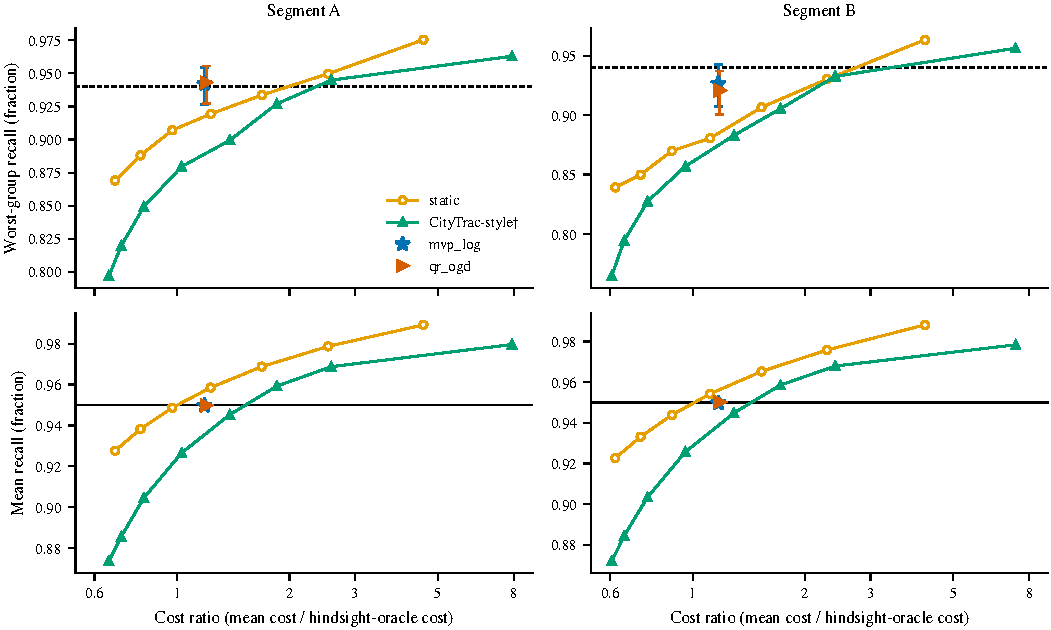
\includegraphics[width=\textwidth]{generated/figures/fig_frontier.pdf}
\caption{Recall against cost on the held-out period (evaluation seed~0;
additional analysis). Curves: \texttt{static} and the CityTrac-style rule with
varying targets. Points: \texttt{mvp\_log} and \texttt{qr\_ogd}; vertical bars
show the 95\% Wilson interval of their worst group (re-acquisition hops); in
segment~A the bars overlap because the two costs nearly coincide. Top: worst-group
recall, dashed line at the bar \groupBar. Bottom: mean recall, line at the target
\targetRecall. Logarithmic cost axis.}
\label{fig:frontier}
\end{figure*}

% =====================================================================
% Supplementary section: reanalysis of the held-out period (David, 2026-10-19)
% Insert into sections/supplementary.tex after the section moved from
% Appendix B (app:heldout). Labels prefixed M- refer to the main manuscript.
% Numbers only through macros (confirm2_numbers.tex); results ccpilot 533850c.
% =====================================================================
\section{Reanalysis of the Held-Out Period in the Confirmation Format}
\label{supp:reanalysis}

After the confirmation results were known, the held-out period of the earlier
evaluation (Appendix~\ref{app:earlier}) was reanalysed with the targets,
estimates, comparators, hindsight references, and decision rules of the
confirmation experiment, as the locked plan specified in advance (Sec.~12 of the
analysis plan). The
earlier per-hop results were reproduced exactly. The reanalysis is an additional
analysis of a period whose results were already known: it checks consistency
between periods and changes no verdict of the confirmation period.

Table~\ref{tab:heldout_reanalysis} lists the verdicts on both periods. The
verdicts on group against marginal calibration (S1) and on online updating
against daily refitting (S2) were the same on both periods.
% CHECK(Alex/Sean): confirm that the S1 main verdict and the S2 verdict are
% identical on both periods; otherwise rewrite this sentence.
Two verdicts differed. Against \texttt{qr\_groups} (S1 addition),
\texttt{mvp\_log} was not distinguished at \ctwoHeldEqualCountQrGroupsMvpLog{} of
five targets, whereas it was worse at \ctwoWorseCountQrGroupsMvpLog{} on the
confirmation period, and \texttt{qr\_ogd} improved on \texttt{qr\_groups} at
\ctwoHeldImprovedCountQrGroupsQrOgd{} of five targets, whereas it was not
distinguished at \ctwoEqualCountQrGroupsQrOgd{} on the confirmation period. In the rarest group (S4), the 95\% lower bound of the re-acquisition shortfall
was above zero at a majority of targets on the held-out period for both online
methods, whereas on the confirmation period this held for \texttt{mvp\_log} only.

The ordering among the group methods therefore changed between the two periods,
and so did the verdict on the rarest group, while their difference from marginal
calibration did not. A change of ordering is
what differences within the variability between periods would produce; it does
not by itself separate sampling variability from a genuine dependence on the
period, and neither period supports a general ranking of the group methods.
Following the plan, the main text reports the verdicts of the confirmation period.

\begin{table*}[!htbp]
\centering
\caption{Verdicts of the decision rules (Sec.~10.8 of the analysis plan) on the confirmation
period and, applied after the confirmation, on the earlier held-out period
(additional analysis; the held-out results were already known). S1: group against
marginal calibration; S1 addition: online methods against \texttt{qr\_groups};
S2: online methods against the refitted variants, one verdict per method, with the number of targets at which the online method was worse given per refitted variant; S4: rarest group, where ``remains'' means that the 95\% lower bound of the re-acquisition shortfall was above zero at a majority of targets and ``qualified'' that it was not. Counts are
over the five targets. The verdict words are those of the locked judgment file
and the counts those of the file of estimates.}
% v4 (judgment 비판01 F6): two sources -- verdict words from claims_10_8.csv,
% counts from main_estimands.csv. Request (Alex): print "qualified" instead of
% "restrict" in tab_heldout_reanalysis.tex (generator).
\label{tab:heldout_reanalysis}
\footnotesize
\IfFileExists{generated/tables/tab_heldout_reanalysis.tex}{% source: results/porto_cctv_confirm2/analysis/claims_10_8.csv @ 1a806b3; results/porto_cctv_confirm2/analysis/main_estimands.csv @ 1a806b3; results/porto_cctv_confirm2/analysis/deficits.csv @ 1a806b3; results/porto_cctv_heldout_reanalysis/analysis/claims_10_8.csv @ 533850c; results/porto_cctv_heldout_reanalysis/analysis/main_estimands.csv @ 533850c; results/porto_cctv_heldout_reanalysis/analysis/deficits.csv @ 533850c
% status = claims_10_8.csv (locked judge; 'restrict (previous evaluation ...)' shown as 'qualified', '반대였다' as 'opposite'; plan statements S1-S4 shown as Claim 1-4); targets = number of the five targets: S1 core improvement against static and against ACI; S1 addition improvement against Mondrian / qr_groups; S2 one verdict per method, worsening count per variant; S4 95% lower bound of the re-acquisition shortfall above zero.
\begin{tabular}{@{}lllrlr@{}}
\toprule
 & & \multicolumn{2}{c}{Confirmation} & \multicolumn{2}{c}{Held-out} \\
\cmidrule(lr){3-4}\cmidrule(l){5-6}
Statement & Method & Judgment & Targets & Judgment & Targets \\
\midrule
Claim 1 & \texttt{mvp\_log} & kept & 5/5 & kept & 5/5 \\
Claim 1 & \texttt{qr\_ogd} & kept & 5/5 & kept & 5/5 \\
Claim 1 addition & \texttt{mvp\_log} & added &  & added &  \\
\quad improved against Mondrian & &  & 5/5 &  & 5/5 \\
\quad improved against \texttt{qr\_groups} & &  & 0/5 &  & 1/5 \\
Claim 1 addition & \texttt{qr\_ogd} & added &  & not added &  \\
\quad improved against Mondrian & &  & 5/5 &  & 5/5 \\
\quad improved against \texttt{qr\_groups} & &  & 0/5 &  & 5/5 \\
Claim 2 & \texttt{mvp\_log} & opposite &  & opposite &  \\
\quad worse than \texttt{qr\_groups\_refit} & &  & 5/5 &  & 4/5 \\
\quad worse than \texttt{qr\_groups\_refit7} & &  & 5/5 &  & 4/5 \\
Claim 2 & \texttt{qr\_ogd} & opposite &  & opposite &  \\
\quad worse than \texttt{qr\_groups\_refit} & &  & 3/5 &  & 3/5 \\
\quad worse than \texttt{qr\_groups\_refit7} & &  & 0/5 &  & 3/5 \\
Claim 4 & \texttt{mvp\_log} & remains & 4/5 & remains & 5/5 \\
Claim 4 & \texttt{qr\_ogd} & qualified & 0/5 & remains & 4/5 \\
\bottomrule
\end{tabular}
}{%
\fbox{\parbox{0.9\textwidth}{\centering tab\_heldout\_reanalysis --- table from Alex}}}
\end{table*}

% =====================================================================
% Supplementary section: confirmation diagnostics and tuning history
% (David, 2026-10-19; moved from Appendix B with JD's approval).
% Insert into sections/supplementary.tex after supp:reanalysis.
% Labels are unchanged; the main text refers to them as S-tab:c2_diagnostics
% and S-tab:c2_tuning. Labels prefixed M- refer to the main manuscript.
% =====================================================================
\section{Confirmation Experiment: Diagnostics and Tuning History}
\label{supp:confirm2diag}

\begin{figure*}[!htbp]
\centering
\IfFileExists{generated/figures/fig_c2_blocks.pdf}{%
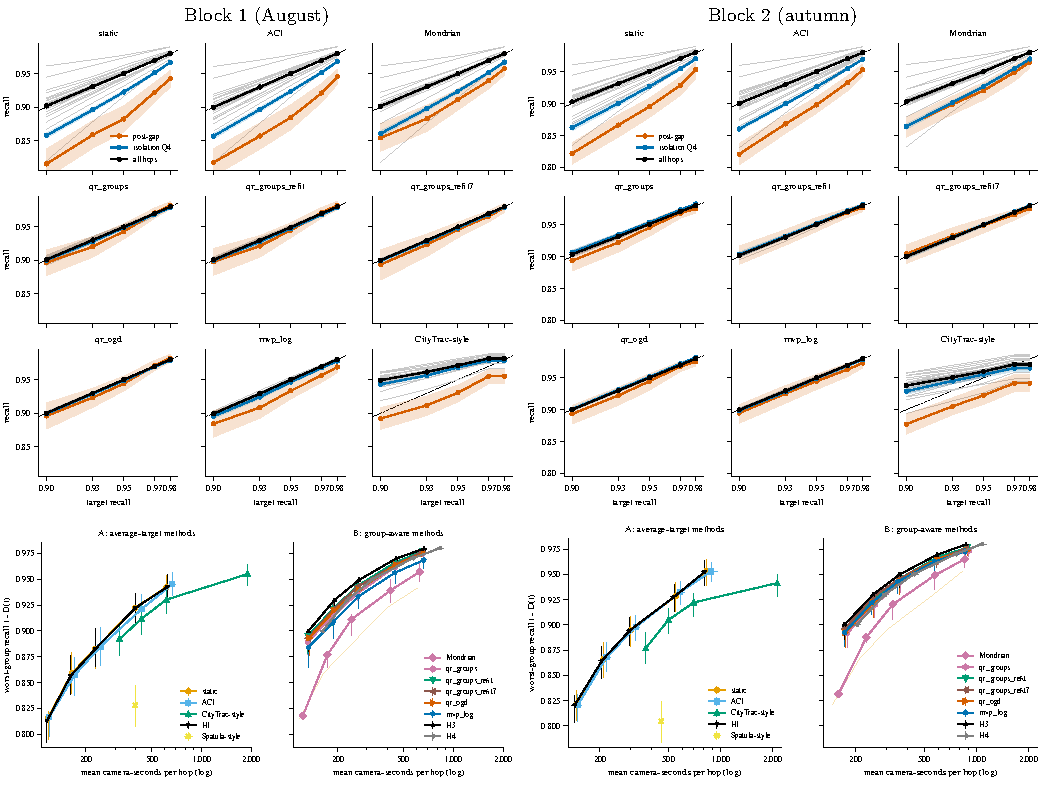
\includegraphics[width=\textwidth]{generated/figures/fig_c2_blocks.pdf}}{%
\fbox{\parbox[c][5cm][c]{0.95\textwidth}{\centering fig\_c2\_blocks --- file from Alex}}}
\caption{Calibration (top) and cost (bottom) on each block of the confirmation
period (left: 5 August to 1 September; right: 7 October to 3 November 2013), drawn
as in Figs.~\ref{M-fig:c2_calibration} and~\ref{M-fig:c2_cost}.}
\label{fig:c2_blocks}
\end{figure*}

\paragraph*{Diagnostics}
Table~\ref{tab:c2_diagnostics} reports, for the confirmation period
(Appendix~\ref{app:confirm2}), the range of $\bar{D}$ and of the re-acquisition
shortfall over the \ctwoNumSeeds{} seeds, three variants of ACI, the share of hops
at which \texttt{mvp\_log} searched at the floor $a_{\min}$ at target 0.98, and
the reachable upper bound of recall in the two groups fixed in advance. Of the
ACI variants, two differ only in the step size; the third is a group-wise ACI
over time of day and first hop (10 cells), which was not a pre-specified
comparator. ACI with separate states per Mondrian cell was not run; a group-wise
ACI over the 25 groups is among the additional baselines of
Section~\ref{M-sec:results:baselines}. Results of \texttt{qr\_ogd} depend on the
seed: at target 0.90, its range over seeds was \ctwoQrOgdSeedSpreadRatio{} of the
width of its interval.
% v4-2 (C8): moved from the limitations of the main text.

\begin{table*}[!htbp]
\centering
\caption{Diagnostics on the confirmation period. Range over seeds of $\bar{D}$
and of the re-acquisition shortfall (pp) and its ratio to the interval width;
three ACI variants ($\gamma=0.0005$; $\gamma=0.001$; group-wise ACI over time of
day $\times$ first hop with $\gamma=0.001$ and floor $\alpha/5$), means over
seeds and blocks without intervals; share of hops at $a_{\min}$ for
\texttt{mvp\_log} at target 0.98; reachable upper bound of recall in the
re-acquisition and isolation~Q4 groups, both blocks pooled.}
\label{tab:c2_diagnostics}
\footnotesize
\IfFileExists{generated/tables/tab_c2_diagnostics.tex}{% source: results/porto_cctv_confirm2/analysis/seed_range.csv @ 1a806b3; results/porto_cctv_confirm2/analysis/group_recall.csv @ 1a806b3; results/porto_cctv_confirm2/analysis/deficits.csv @ 1a806b3; results/porto_cctv_confirm2/runs/<block>/t<target>/s<seed>/summary.csv @ untracked; results/porto_cctv_confirm2/analysis/a_min_reach.csv @ 1a806b3; results/porto_cctv_confirm2/analysis/reachable_bound.csv @ 1a806b3
% (a) Dbar: seed_range.csv D_seed_min-D_seed_max (seed_range_over_ci_width); re-acquisition: min-max over seeds of group_recall.csv deficit (hopkind=2), ratio = range / (hi - lo) of deficits.csv; (b) ACI variants: run summaries (coverage, as-run worst group, cost; seed means per block; no interval); (c) a_min_reach.csv target 0.98; (d) reachable_bound.csv U_G.
\setlength{\tabcolsep}{3.2pt}
\begin{tabular}{@{}llrrrrr@{}}
\toprule
Method & Quantity & 0.90 & 0.93 & 0.95 & 0.97 & 0.98 \\
\midrule
\multicolumn{7}{@{}l}{\emph{(a) Range over the 5 seeds, pp (ratio to the 95\% interval width)}} \\
\texttt{mvp\_log} & \Dbar{} & 0.8--1.3 (0.32) & 0.8--1.7 (0.52) & 0.5--1.4 (0.67) & 0.7--1.2 (0.42) & 0.6--1.1 (0.40) \\
 & Post-gap $d$ & 0.8--1.3 (0.23) & 0.8--1.7 (0.42) & 0.5--1.4 (0.54) & 0.7--1.2 (0.40) & 0.6--1.1 (0.38) \\
\texttt{qr\_ogd} & \Dbar{} & 0.2--1.4 (0.79) & 0.2--1.5 (0.78) & 0.2--1.2 (0.80) & 0.1--1.1 (1.92) & 0.1--1.0 (1.49) \\
 & Post-gap $d$ & $-$0.3--1.4 (0.74) & $-$0.4--1.5 (0.91) & $-$0.1--1.2 (0.74) & $-$0.7--1.1 (1.69) & $-$0.5--1.0 (1.62) \\
\texttt{static} & \Dbar{} & 8.1--8.1 (0.00) & 6.7--6.7 (0.00) & 6.0--6.0 (0.00) & 4.4--4.4 (0.00) & 3.1--3.1 (0.00) \\
 & Post-gap $d$ & 8.1--8.1 (0.00) & 6.7--6.7 (0.00) & 6.0--6.0 (0.00) & 4.4--4.4 (0.00) & 3.1--3.1 (0.00) \\
ACI & \Dbar{} & 7.8--8.2 (0.19) & 6.4--6.8 (0.19) & 5.6--5.9 (0.17) & 4.2--4.3 (0.09) & 2.9--3.1 (0.19) \\
 & Post-gap $d$ & 7.8--8.2 (0.15) & 6.4--6.8 (0.19) & 5.6--5.9 (0.17) & 4.2--4.3 (0.09) & 2.9--3.1 (0.19) \\
Mondrian & \Dbar{} & 7.4--7.4 (0.00) & 4.7--4.7 (0.00) & 3.3--3.3 (0.00) & 2.5--2.5 (0.00) & 1.8--1.8 (0.00) \\
 & Post-gap $d$ & 4.0--4.0 (0.00) & 3.8--3.8 (0.00) & 3.3--3.3 (0.00) & 2.5--2.5 (0.00) & 1.8--1.8 (0.00) \\
\texttt{qr\_groups} & \Dbar{} & 0.4--1.3 (0.64) & 0.4--1.7 (0.89) & 0.3--1.2 (0.81) & 0.2--1.2 (2.03) & 0.2--1.0 (1.60) \\
 & Post-gap $d$ & $-$0.6--1.3 (0.82) & $-$0.5--1.7 (1.06) & $-$0.2--1.2 (0.81) & $-$0.7--1.2 (1.74) & $-$0.5--1.0 (1.66) \\
\texttt{qr\_groups\_refit} & \Dbar{} & 0.2--0.3 (0.09) & 0.3--0.5 (0.22) & 0.2--0.4 (0.21) & 0.1--0.3 (0.41) & 0.1--0.3 (0.46) \\
 & Post-gap $d$ & $-$0.4--0.1 (0.22) & 0.0--0.5 (0.27) & $-$0.2--0.4 (0.37) & $-$0.2--0.3 (0.52) & 0.0--0.3 (0.34) \\
\texttt{qr\_groups\_refit7} & \Dbar{} & 0.1--0.8 (0.61) & 0.1--0.6 (0.40) & 0.2--0.8 (0.60) & 0.1--0.8 (0.83) & 0.1--0.6 (0.72) \\
 & Post-gap $d$ & $-$0.6--0.8 (0.60) & $-$0.8--0.6 (0.67) & $-$0.9--0.8 (1.01) & $-$0.2--0.8 (0.91) & 0.1--0.6 (0.56) \\
CityTrac-style & \Dbar{} & 1.7--1.7 (0.00) & 2.2--2.2 (0.00) & 2.4--2.4 (0.00) & 2.3--2.3 (0.00) & 3.3--3.3 (0.00) \\
 & Post-gap $d$ & 1.7--1.7 (0.00) & 2.2--2.2 (0.00) & 2.4--2.4 (0.00) & 2.3--2.3 (0.00) & 3.3--3.3 (0.00) \\
Spatula-style & \Dbar{} & 8.6--8.6 (0.00) & 11.6--11.6 (0.00) & 13.6--13.6 (0.00) & 15.6--15.6 (0.00) & 16.6--16.6 (0.00) \\
 & Post-gap $d$ & 8.6--8.6 (0.00) & 11.6--11.6 (0.00) & 13.6--13.6 (0.00) & 15.6--15.6 (0.00) & 16.6--16.6 (0.00) \\
\midrule
\multicolumn{7}{@{}l}{\emph{(b) ACI variants (mean over seeds and the two blocks; no interval): recall / worst group / cost}} \\
ACI $\gamma=0.0005$ (main) & recall / worst / cost & 0.900 / 0.819 / 135 & 0.930 / 0.863 / 195 & 0.950 / 0.891 / 284 & 0.970 / 0.927 / 509 & 0.980 / 0.949 / 774 \\
ACI $\gamma=0.001$ & recall / worst / cost & 0.900 / 0.818 / 136 & 0.930 / 0.863 / 197 & 0.950 / 0.893 / 289 & 0.970 / 0.927 / 516 & 0.980 / 0.949 / 800 \\
ACI per time of day $\times$ first hop & recall / worst / cost & 0.900 / 0.822 / 135 & 0.930 / 0.880 / 196 & 0.950 / 0.914 / 283 & 0.970 / 0.944 / 496 & 0.980 / 0.962 / 767 \\
\midrule
\multicolumn{7}{@{}l}{\emph{(c) \texttt{mvp\_log} hops at $a_{\min}$, target 0.98, seeds 0--4 (\%): 0.0058, 0.0071, 0.0086, 0.0094, 0.0100}} \\
\multicolumn{7}{@{}l}{\emph{(d) Reachable upper bound of recall $U_G$: post-gap 0.9998, isolation Q4 0.9998}} \\
\bottomrule
\end{tabular}
}{%
\fbox{\parbox{0.9\textwidth}{\centering tab\_c2\_diagnostics --- table from Alex}}}
\end{table*}

\paragraph*{Trial run and tuning history}
Before the lock, the full pipeline was run once on exploratory period~1 to check
it (Sec.~13.8 of the analysis plan). The check of detection times failed in that run, and the
recording code was corrected (commit \texttt{b5e10e6}); no method, comparator, or
decision rule was changed after the trial run, and the comparators were defined
before it. Table~\ref{tab:c2_tuning} lists, for each method, the parameters, how
and on which period they were chosen, and the trial-run values ($\bar{D}$ and the
cost ratio to H1 at target 0.95, seeds 0 and 1).

\begin{table*}[!htbp]
\centering
\caption{Tuning history of each method (parameters, and how and on which period
they were chosen) and the trial run on exploratory period~1 before the lock
($\bar{D}$ in pp and cost ratio to H1, target 0.95, seeds 0 and 1). The history
before the pre-registration tag is taken from the research notes of that time
and cannot be verified from the version history. After the trial run, only the
recording code was corrected (\texttt{b5e10e6}); no method, comparator, or
decision rule was changed.}
\label{tab:c2_tuning}
\footnotesize
\IfFileExists{generated/tables/tab_c2_tuning.tex}{% source: results/precheck_confirm2/precheck_report2.md @ 71193cd; results/precheck_confirm2/trial_expl1/analysis/group_recall.csv @ 7d954a1; results/precheck_confirm2/trial_expl1/analysis/cost_ratios.csv @ 7d954a1; configs/porto_cctv_confirm2.yaml @ 6758bce
% tuning history: precheck_report2.md section A9 (research records README v2-v7; before the pre-registration tag, not verifiable in git), translated; refit variants: plan section 3 and commit dcc7f9f; baseline parameters: run config. Trial: exploratory period 1, target 0.95, evaluation seeds 0-1; Dbar = 0.95 - min over the judged groups of the seed-mean recall (pp); cost ratio to H1 (cost_ratios.csv point). CityTrac-style at nominal 0.95.
\setlength{\tabcolsep}{3pt}
\begin{tabular}{@{}lp{6.2cm}p{3.6cm}lrr@{}}
\toprule
 & & & & \multicolumn{2}{c}{Trial run} \\
\cmidrule(l){5-6}
Method & Tuned parameters & Chosen on & Variants & \Dbar{} (pp) & Cost/H1 \\
\midrule
\texttt{static} & none & -- & -- & 6.5 & 0.91 \\
ACI & $\gamma \in \{0.005, 0.001, 0.0005\}$, floor $\alpha/5$, per hour $\times$ first hop; window 2{,}000 (initial value) & expl.\ 1 (virtual layout), then expl.\ 2 (virtual) & 5, then 3 kept & 5.5 & 1.07 \\
Mondrian & cells (hour, first hop, hour $\times$ first hop; later speed and hour $\times$ first hop $\times$ speed, 40 cells); minimum 200 & expl.\ 1, then expl.\ 2 (virtual) & 5 & 3.9 & 0.98 \\
\texttt{qr\_groups} & log scale (linear scale gave negative $\tau$); at most 80{,}000 rows & exploratory & 2 scales & 3.8 & 1.08 \\
\texttt{qr\_groups\_refit} & as \texttt{qr\_groups}, refitted daily, cumulative & defined before the trial run & 1 & 0.9 & 1.10 \\
\texttt{qr\_groups\_refit7} & as \texttt{qr\_groups}, refitted daily, 7-day window & defined before the trial run & 1 & 0.2 & 1.16 \\
\texttt{qr\_ogd} & $\gamma = 0.005$, clip 3 & exploratory & 1 & 2.6 & 1.16 \\
\texttt{mvp\_log} & log scale, $a_{\min} = 0.002$, $m = 40$ & expl.\ 1 and 2 (real layout) & 1 & 1.3 & 1.15 \\
Spatula-style & share threshold 0.05, delay quantile 0.98 & from the reading of the paper & -- & 16.1 & 1.48 \\
CityTrac-style & delay window quantile 0.98, minimum 30 per key & from the reading of the paper & -- & 3.7 & 2.24 \\
\midrule
Predictor & hierarchy src $\to$ zone $\to$ hour $\to$ speed; $\lambda = 20$, $\varepsilon = 10^{-4}$, $\sigma = 1$ bin & expl.\ 1 and 2 & 5 & & \\
Groups, criteria & 25 groups; bar 0.94 (first draft); cost bound 1.20 & research records & -- & & \\
\midrule
Trial run (pre-lock) & detection-time output compared in float64 like the score (the first trial run stopped on the consistency check); output code only, no method, comparator, or parameter changed (commit \texttt{b5e10e6}) & exploratory period 1 & -- & & \\
\bottomrule
\end{tabular}

\smallskip\parbox{\textwidth}{\footnotesize Tuning history before the pre-registration tag (\texttt{prereg-v3}): research records (README versions 2--7 and internal deviation notes), not verifiable in the version history. Trial run: exploratory period 1, target 0.95, evaluation seeds 0--1, made before the lock of the confirmation plan.}
}{%
\fbox{\parbox{0.9\textwidth}{\centering tab\_c2\_tuning --- table from Alex}}}
\end{table*}

% =====================================================================
% v4-5 (David, 2026-10-22): additional analyses added during revision
% (feedback and predictor sensitivity). Tables from Alex (review02).
% =====================================================================
\section{Additional Analyses Added During Revision}
\label{supp:review}

The analyses in this section were added during revision, after the
confirmation results were known, with a plan fixed before any aggregate was
computed; the main text discusses them in Section~\ref{M-sec:discussion}.

\begin{table*}[!htbp]
\centering
\caption{Feedback sensitivity on the confirmation period (target 0.95, both
blocks pooled, mean over seeds): worst-group shortfall $\bar{D}$ and
re-acquisition shortfall (pp), and cost relative to H2, with conservative 95\%
intervals. Label sets (i)--(iv) as in Section~\ref{M-sec:discussion}. The refit
reads only labelled scores, so its rows for (iii) and (iv) equal those for (i)
and (ii). A threshold above every predicted probability searches nothing and costs zero.}
% v4-6: this states the cost definition used after the correction of the cost
% lookup (Alex report 03, c7de4f7; REVIEW deviation R3).
\label{tab:review_feedback}
\footnotesize
\IfFileExists{generated/tables/tab_review_feedback.tex}{% POST HOC (added during revision (internal review)), generated by posthoc_review_tables.py; confirmation period, both blocks, target 0.95, seeds 0-4 (mean), primary predictor; D and re-acquisition d in pp; [95% interval, taxi and day cluster bootstraps, B = 2,000, conservative]; rows (v) and 7-day refit under (iv): review/B_v_estimates.csv (methods v_aci_groups, v_mvp_log, v_qr_ogd, Biv_refit7_a; the 7-day refit row at target 0.93 is at 0.93)
\begin{tabular}{@{}llccc@{}}
\toprule
Label set & Method & $\bar{D}$ & Post-gap $d$ & Cost / H2 \\
\midrule
full & ACI & 5.7 [4.7, 6.8] & 5.7 [4.7, 6.8] & 1.08 [1.07, 1.09] \\
 & group-wise ACI & 0.1 [$-$0.0, 0.8] & $-$0.1 [$-$0.9, 0.8] & 1.10 [1.08, 1.11] \\
 & mvp\_log & 1.0 [0.5, 1.9] & 1.0 [0.2, 1.9] & 1.18 [1.17, 1.19] \\
 & qr\_ogd & 0.7 [0.2, 1.5] & 0.6 [$-$0.2, 1.5] & 1.20 [1.18, 1.21] \\
 & refit & 0.3 [0.2, 1.0] & 0.2 [$-$0.6, 1.0] & 1.18 [1.17, 1.20] \\
\addlinespace
(i) & ACI & 5.5 [4.5, 6.5] & 5.5 [4.5, 6.5] & 5.40 [5.10, 5.73] \\
 & mvp\_log & 1.0 [0.5, 1.9] & 1.0 [0.2, 1.9] & 1.18 [1.17, 1.19] \\
 & qr\_ogd & 0.7 [0.2, 1.5] & 0.6 [$-$0.2, 1.5] & 1.20 [1.18, 1.21] \\
 & refit & 2.4 [2.1, 3.3] & 2.2 [1.2, 3.3] & 1.23 [1.21, 1.24] \\
\addlinespace
(ii) & ACI & 5.7 [4.7, 6.7] & 5.7 [4.7, 6.7] & 1.23 [1.17, 1.31] \\
 & mvp\_log & 1.1 [0.5, 2.0] & 1.1 [0.3, 2.0] & 1.18 [1.17, 1.19] \\
 & qr\_ogd & 0.7 [0.2, 1.5] & 0.6 [$-$0.2, 1.5] & 1.20 [1.18, 1.21] \\
 & refit & 2.1 [1.8, 2.9] & 1.9 [0.9, 2.9] & 1.22 [1.21, 1.23] \\
\addlinespace
(iii) & ACI & 91.7 [88.6, 94.2] & 90.6 [86.8, 93.4] & 3.93 [1.41, 5.61] \\
 & group-wise ACI & 69.8 [63.8, 75.4] & 3.0 [2.0, 4.1] & 2.39 [1.78, 3.09] \\
 & mvp\_log & 86.4 [81.5, 91.6] & 21.4 [16.6, 26.6] & 25.33 [17.61, 36.09] \\
 & qr\_ogd & 93.0 [90.4, 94.8] & 33.8 [30.5, 37.0] & 16.95 [10.51, 21.13] \\
 & refit$^a$ & 2.4 [2.1, 3.3] & 2.2 [1.2, 3.3] & 1.23 [1.21, 1.24] \\
\addlinespace
(iv) & ACI & 40.5 [39.7, 41.3] & 33.2 [31.3, 35.1] & 1.03 [1.02, 1.05] \\
 & group-wise ACI & 20.8 [19.7, 21.8] & 2.6 [1.6, 3.8] & 1.10 [1.04, 1.17] \\
 & mvp\_log & 22.3 [20.8, 23.7] & 17.2 [15.0, 19.5] & 1.27 [1.17, 1.38] \\
 & qr\_ogd & 21.8 [21.5, 22.5] & 6.2 [5.1, 7.4] & 1.31 [1.23, 1.41] \\
 & refit$^a$ & 2.1 [1.8, 2.9] & 1.9 [0.9, 2.9] & 1.22 [1.21, 1.23] \\
 & seven-day refit$^c$, target 0.95 & 9.0 [7.7, 10.5] & 8.1 [6.4, 9.8] & 1.43 [1.33, 1.51] \\
 & seven-day refit$^c$, target 0.93 & 11.9 [10.2, 14.0] & 11.4 [9.2, 13.5] & 1.39 [1.31, 1.46] \\
\addlinespace
(v)$^b$ & group-wise ACI & 0.3 [0.0, 1.1] & 0.1 [$-$0.7, 1.1] & 1.03 [1.02, 1.04] \\
 & mvp\_log & 1.6 [0.8, 2.7] & 1.6 [0.7, 2.7] & 1.17 [1.16, 1.18] \\
 & qr\_ogd & 0.8 [0.4, 1.6] & 0.6 [$-$0.2, 1.6] & 1.20 [1.19, 1.21] \\
\addlinespace
\bottomrule
\end{tabular}

\smallskip\parbox{\linewidth}{\footnotesize $^a$(iii)/(iv) refit = (i)/(ii) refit by construction (the refit reads only labeled scores). $^b$(v): audit hops only, plan revision 5. $^c$\texttt{qr\_groups\_refit7} under (iv), plan revision 5; the 0.93 row by the additional-target rule (plan revision 3).}
}{%
\fbox{\parbox{0.9\textwidth}{\centering tab\_review\_feedback --- table from Alex (REVIEW B)}}}
\end{table*}

\begin{table*}[!htbp]
\centering
\caption{Predictor sensitivity on the confirmation period (target 0.95, both
blocks pooled, mean over seeds): worst-group shortfall $\bar{D}$ and
re-acquisition shortfall (pp), and cost relative to the H2 of the same
predictor, with conservative 95\% intervals.}
\label{tab:review_predictors}
\footnotesize
\IfFileExists{generated/tables/tab_review_predictors.tex}{% POST HOC (added during revision (internal review)), generated by posthoc_review_tables.py; confirmation period, both blocks, target 0.95, seeds 0-4 (mean); D and re-acquisition d in pp; [95% interval, taxi and day cluster bootstraps, B = 2,000, conservative]
\begin{tabular}{@{}llccc@{}}
\toprule
Predictor & Method & $\bar{D}$ & Post-gap $d$ & Cost / H2 \\
\midrule
source site & \texttt{static} & 6.0 [4.8, 7.2] & 6.0 [4.8, 7.2] & 1.00 [1.00, 1.00] \\
 & \texttt{ACI} & 6.1 [5.1, 7.2] & 6.1 [5.1, 7.2] & 1.05 [1.04, 1.06] \\
 & \texttt{Mondrian (40 cells)} & 3.2 [2.7, 4.2] & 3.2 [2.3, 4.2] & 1.02 [1.01, 1.02] \\
 & \texttt{qr\_groups} & 0.6 [0.3, 1.1] & 0.3 [$-$0.4, 1.0] & 1.10 [1.08, 1.11] \\
 & \texttt{mvp\_log} & 0.8 [0.4, 1.6] & 0.8 [0.1, 1.6] & 1.06 [1.05, 1.06] \\
 & \texttt{qr\_ogd} & 0.6 [0.3, 1.1] & 0.3 [$-$0.3, 1.1] & 1.10 [1.09, 1.11] \\
\addlinespace
+ exit zone & \texttt{static} & 6.0 [5.0, 7.2] & 6.0 [5.0, 7.2] & 1.00 [1.00, 1.00] \\
 & \texttt{ACI} & 5.8 [4.8, 6.9] & 5.8 [4.8, 6.9] & 1.06 [1.05, 1.07] \\
 & \texttt{Mondrian (40 cells)} & 3.6 [2.8, 4.6] & 3.6 [2.7, 4.6] & 1.04 [1.03, 1.05] \\
 & \texttt{qr\_groups} & 0.6 [0.3, 1.2] & 0.4 [$-$0.3, 1.1] & 1.12 [1.10, 1.13] \\
 & \texttt{mvp\_log} & 1.3 [0.5, 2.3] & 1.3 [0.4, 2.3] & 1.10 [1.09, 1.11] \\
 & \texttt{qr\_ogd} & 0.5 [0.2, 1.2] & 0.5 [$-$0.2, 1.2] & 1.13 [1.12, 1.14] \\
\addlinespace
+ exit zone, time of day & \texttt{static} & 6.3 [5.2, 7.5] & 6.3 [5.2, 7.5] & 1.00 [1.00, 1.00] \\
 & \texttt{ACI} & 6.0 [5.0, 7.0] & 6.0 [5.0, 7.0] & 1.07 [1.06, 1.08] \\
 & \texttt{Mondrian (40 cells)} & 3.5 [2.8, 4.6] & 3.5 [2.5, 4.6] & 1.06 [1.06, 1.07] \\
 & \texttt{qr\_groups} & 1.2 [0.6, 2.0] & 1.0 [0.2, 2.0] & 1.15 [1.14, 1.16] \\
 & \texttt{mvp\_log} & 1.0 [0.5, 1.9] & 1.0 [0.1, 1.9] & 1.15 [1.14, 1.16] \\
 & \texttt{qr\_ogd} & 1.0 [0.4, 1.9] & 0.9 [0.2, 1.9] & 1.17 [1.16, 1.18] \\
\addlinespace
+ exit zone, exit speed & \texttt{static} & 5.8 [4.7, 7.1] & 5.8 [4.7, 7.1] & 1.00 [1.00, 1.00] \\
 & \texttt{ACI} & 5.6 [4.5, 6.6] & 5.6 [4.5, 6.6] & 1.07 [1.06, 1.08] \\
 & \texttt{Mondrian (40 cells)} & 3.2 [2.9, 4.3] & 3.2 [2.2, 4.3] & 1.07 [1.06, 1.07] \\
 & \texttt{qr\_groups} & 0.4 [0.2, 0.9] & 0.1 [$-$0.7, 0.9] & 1.17 [1.16, 1.18] \\
 & \texttt{mvp\_log} & 1.2 [0.5, 2.1] & 1.2 [0.3, 2.1] & 1.15 [1.14, 1.16] \\
 & \texttt{qr\_ogd} & 0.3 [0.1, 1.1] & 0.2 [$-$0.6, 1.1] & 1.18 [1.17, 1.19] \\
 & \texttt{qr\_groups\_refit} & 0.3 [0.2, 0.9] & 0.1 [$-$0.7, 0.9] & 1.16 [1.15, 1.17] \\
\addlinespace
+ exit zone, time, speed (main) & \texttt{static} & 6.0 [4.9, 7.2] & 6.0 [4.9, 7.2] & 1.00 [1.00, 1.00] \\
 & \texttt{ACI} & 5.7 [4.7, 6.8] & 5.7 [4.7, 6.8] & 1.08 [1.07, 1.09] \\
 & \texttt{Mondrian (40 cells)} & 3.3 [3.0, 4.4] & 3.3 [2.4, 4.4] & 1.08 [1.08, 1.09] \\
 & \texttt{qr\_groups} & 0.8 [0.3, 1.5] & 0.6 [$-$0.2, 1.5] & 1.18 [1.17, 1.19] \\
 & \texttt{mvp\_log} & 1.0 [0.5, 1.9] & 1.0 [0.2, 1.9] & 1.18 [1.17, 1.19] \\
 & \texttt{qr\_ogd} & 0.7 [0.2, 1.5] & 0.6 [$-$0.2, 1.5] & 1.20 [1.18, 1.21] \\
 & \texttt{qr\_groups\_refit} & 0.3 [0.2, 1.0] & 0.2 [$-$0.6, 1.0] & 1.18 [1.17, 1.20] \\
\addlinespace
\bottomrule
\end{tabular}
}{%
\fbox{\parbox{0.9\textwidth}{\centering tab\_review\_predictors --- table from Alex (REVIEW C)}}}
\end{table*}
